
%\documentclass{article}
%\documentclass{ctexart}
\documentclass{sicnuthesis}

%\usepackage[UTF8]{ctex}


\usepackage{graphicx}
\usepackage{hyperref}
\usepackage{amsmath}
\usepackage{algorithm}
\usepackage{algpseudocode}
\usepackage{subcaption}
\usepackage{booktabs}

\usepackage[round]{natbib} % 提供\citet命令把[1]式引用换成(Zhuo 1995)式引用

\usepackage{verbatim} % for block comment

\usepackage[section]{placeins} %强制浮动图片在section内被解决




% For importing python source code, from https://tex.stackexchange.com/questions/83882/how-to-highlight-python-syntax-in-latex-listings-lstinputlistings-command

\usepackage{color}
\definecolor{deepblue}{rgb}{0,0,0.5}
\definecolor{deepred}{rgb}{0.6,0,0}
\definecolor{deepgreen}{rgb}{0,0.5,0}

% Default fixed font does not support bold face
\DeclareFixedFont{\ttb}{T1}{txtt}{bx}{n}{12} % for bold
\DeclareFixedFont{\ttm}{T1}{txtt}{m}{n}{12}  % for normal
\DeclareFixedFont{\ttfuck}{T1}{txtt}{m}{n}{12}  % for normal


\usepackage{listings}

% Python style for highlighting
\newcommand\pythonstyle{\lstset{
language=Python,
basicstyle=\ttm,
otherkeywords={self},             % Add keywords here
keywordstyle=\ttb\color{deepblue},
emph={MyClass,__init__},          % Custom highlighting
emphstyle=\ttb\color{deepred},    % Custom highlighting style
stringstyle=\color{deepgreen},
frame=tb,                         % Any extra options here
showstringspaces=false,             
breaklines=true,                 % come from https://tex.stackexchange.com/questions/243500/python-code-block-outside-of-margin
}}


% Python environment
\lstnewenvironment{python}[1][]
{
\pythonstyle
\lstset{#1}
}
{}

% Python for external files
\newcommand\pythonexternal[2][]{{
\pythonstyle
\lstinputlisting[#1]{#2}}}

% Python for inline
\newcommand\pythoninline[1]{{\pythonstyle\lstinline!#1!}}



\graphicspath{{images/}}

%在sicnuthesis模板中下面都相当于在定义学校那个丑爆的封面

\title{使用贝叶斯方法探测隐藏敌人状态}
\author{卓越羿}
\school{数学与软件科学学院}
\major{统计学}
\class{2014级8班}
\studentid{2014060843}
\tutor{张欣哲}
\date{2018}

\begin{document}

\frontmatter %页码设为罗马数字

\maketitle

\clearpage

\begin{abstractch}

假设一个位置离敌我双方单位越近,则有更高的爆发一场战斗的概率。如果我们
只能观测到友方和战斗发生的位置,应当如何推断敌方单位的位置?
这种隐变量推断问题需要一个设定恰当的正向生成概率模型和有效的算法进行进行反向推断。
本文提出几个战役模型以及编写了一个基于pytorch的贝叶斯推断框架,并将它们应用到点和运动探测,
存在概率估计上,并分别使用了均匀先验和其他数据相关的先验。同时也都使用了不同
的初始值测试算法的有效性。文章最后包含一个葛底斯堡战役的案例研究覆盖全文讨论的内容。
\footnote{LaTeX代码(英/中文)和实验文件已经托管在GitHub,见: \url{ https://github.com/yiyuezhuo/Undergraduate-thesis } 。原文以英语写成,受制于学校规定翻译成了中文}

\end{abstractch}

\begin{keywordsch}贝叶斯统计;变分推断;马尔科夫蒙特卡洛\end{keywordsch}

\clearpage


\begin{abstracten}

Assuming a location which have samller distance to two conflict factions have higher probability causing a battle,
how do we infer the location of enemy if we can only observe the locations of allies and battles? 
The latent variable inference problem requieres a suitable front probability model and a effiecent way to run the 
inference. In this work, a battle model is introduced and a bayes inference framework based on pytorch 
is developed to reach the inference task including point, movement detection and 
exist probability estimation with different prior and various initialization value setting.
A case study about The battle of Gettysburg is included to show the overview of the content covered by the paper.

\end{abstracten}

\begin{keywordsen}bayes statistic;variational inference;MCMC\end{keywordsen}


\clearpage

\tableofcontents

\clearpage

\mainmatter %页码设为阿拉伯数字

\section{绪论}

在真实战场上,你不能像RTS和经典桌上兵棋那样直接观测到敌方单位,甚至连友方单位都不能观测到。
你能依赖的唯一的东西就是那些混乱复杂乃至自相矛盾的信息和谣言。有很多因为错误信息导致失败的例子,
如孙膑减灶愚弄对手,麦克莱伦将军因为南方军设的“和平炮”
\footnote{下文将经常提到美国内战的例子,特别是葛底斯堡战役作为案例研究,
这是因为作者曾长时间推演HPS内战/拿破仑系列兵棋。对此比较了解}(装扮成炮的道具)而驻兵不前,
从而失去一举击败邦联的机会。

不幸的是,当前军事决策模拟程序,如经典兵棋(一个例子可见图~\ref{fig:hps})和某些“严肃”RTS,
总是试图去捕捉更“宏大”的层面(倒也许和他们荒谬的热衷于宏大叙事历史学同行不同),而对侦查和信息使用
这类难以难以建模又并不有趣的东西避之不及,乃至采用了过度的简化。

\begin{figure}[htb]
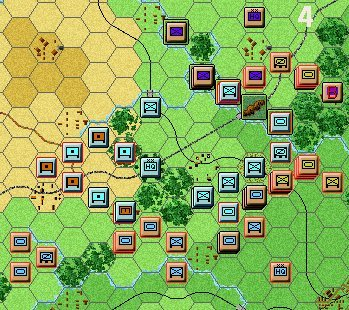
\includegraphics[width=0.6\linewidth]{SmolenskR4.jpg}
\caption{
图中展示了经典兵棋公司HPS的作品斯摩棱斯克41对侦查的处理——单位仅能出于完全可知和完全不可知的状态。 }
\label{fig:hps}
\end{figure}


尽管我们经常可以直接在事后画的战场局势图上看到战斗序列(即那些方框图标),如图~\ref{fig:metz}所示。
但是显然这些标记是根据事后对照双方信息才得以制成的,在真实战场上,我们并不能指望某些像“地图模拟软件”
那样看到敌人踪迹,甚至还能看到明显不应该能精确观测到的量化信息。真的传达的到的很可能是错的或者误导信息。
杰克逊将军在谷地利用迷惑性行动使得林肯政府和指挥手足无措就是个生动的例子。


\begin{figure}[htb]
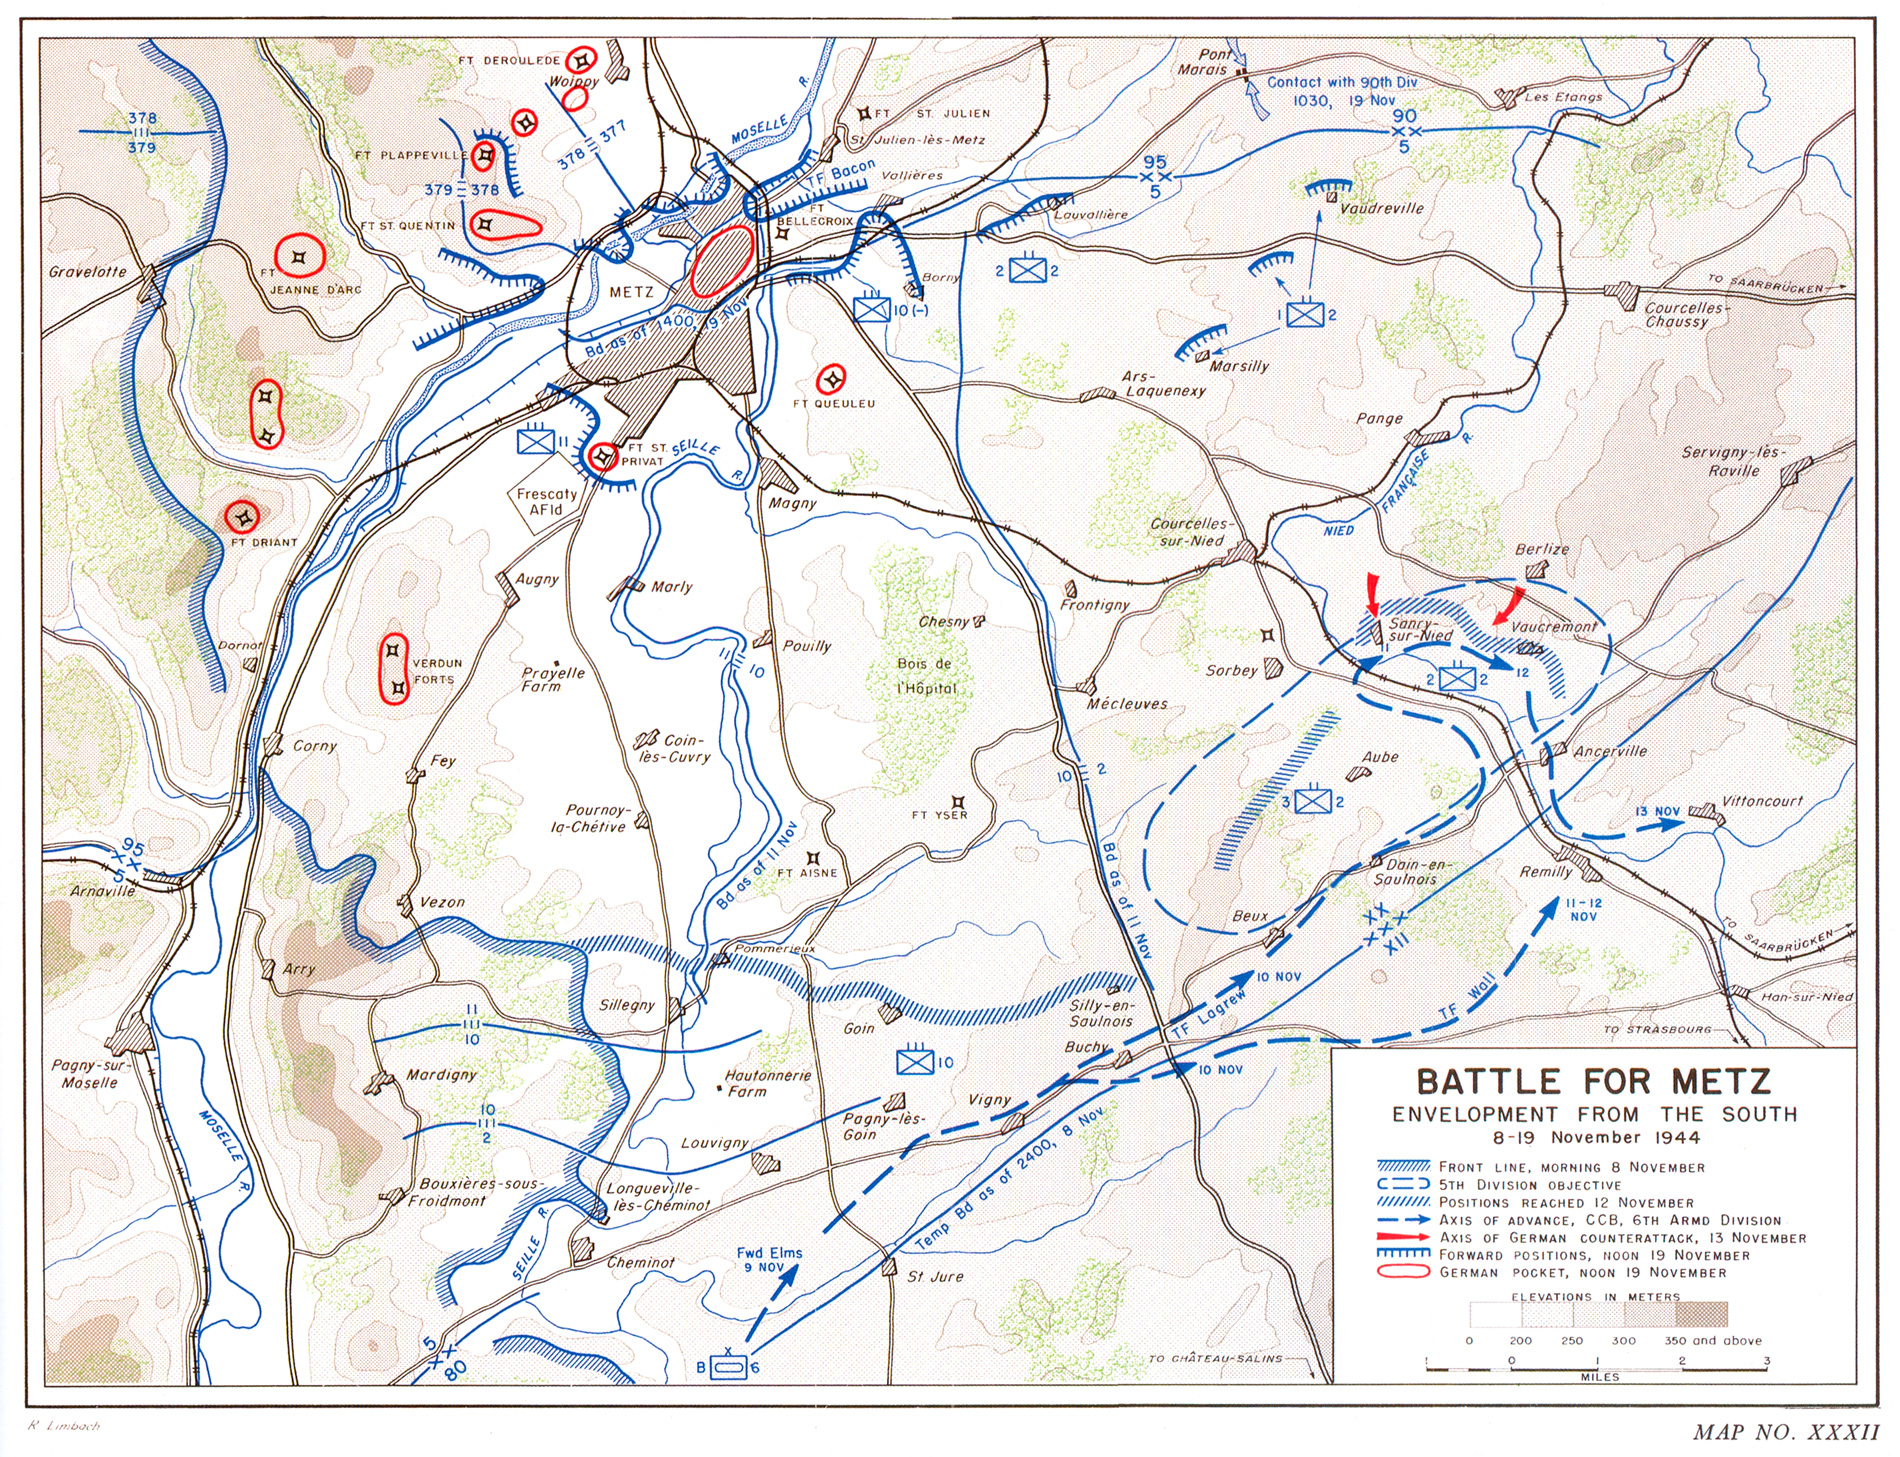
\includegraphics[width=0.6\linewidth]{metz.jpg}
\caption{
梅兹战役地图,地图展示了并不应该在真实战场上所能看到的OOB }
\label{fig:metz}
\end{figure}

\subsection{相关工作}

已经有一些工作致力于解决这一信息处理方式过于简单暴力的问题,如
\cite{hostetler2012inferring} \cite{vsmejkal2016integrating} \cite{touhou}。
这些工作手动将完全信息中的一大部分屏蔽,虽然这种屏蔽类似特征工程所做的,但目的并非使得算法更有效,
而是手动模拟出一个信息不完全环境来测试一些处理算法。不过总的来说它们并不是很有用。本文将以
一种更直接,直觉的方式解决这个问题,主要围绕位置和运动的探测展开。


\clearpage
\section{构建正向生成模型}

\subsection{简单模型}

在正向生成模型中,可以定义一个二维随机点过程,首先抽一个战役数量,然后独立同分布的从一个二维分布中
抽取那个数量的战役坐标。例如,给定如图~\ref{fig:stateNoBattle}所示友军和敌军的地点位置:

\begin{figure}[htb]
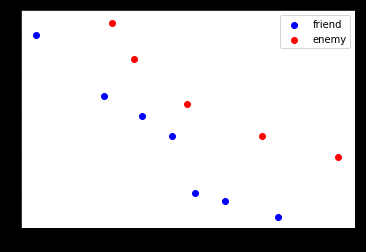
\includegraphics{state_no_battle.png}
\caption{
友军和敌军的位置设定}
\label{fig:stateNoBattle}
\end{figure}


假定战役数是$10$\footnote{这是为了简化,后文的战役数都是给定的而不是随机过程的一部分。}
于是可设这$10$个战役是从下述分布所抽取出来的:

$$
P(x,y) \propto \max_i p^A_{i}(x,y) \max_j p^E_{j} (x,y)
$$


这里 $p^A_{i}(x,y)$ 表示第$i$个友方单位“散布”出来的概率密度,
$p^E_{j}$ 表示第$j$个敌方单位单位对应的密度。这个密度又被定义为:


$$
P^S_i(x,y) \propto \exp(-\frac{1}{2}((x-x^S_i)^2 + (y-y^S_i)^2))
$$


表示$S$方($S \in \{A,E  \}$)第$i$个单位在点$(x,y)$释放的概率。故而上式可被重写为: 

$$
P(x,y) \propto \exp(-\frac{1}{2}((x-x_{nearst(x,y)})^2 + (y-y_{nearst(x,y)})^2))
$$

这里$nearst(x,y)$表示离点$(x,y)$最近的单位(敌方或友方)。

这么定义使得此非标准化概率仅仅被决定于两个最近的冲突单位的距离。这个来自两个单位在以其为位置为中心的
区域内漫游而碰撞的自然推导,不过它们是独立的抽出来等假设显然是不对的。之后这个模型会被修改和比较。

无论如何,现在标准化概率可以被计算出来并如等高线图~\ref{fig:stateNoBattleProb}所示。

\begin{figure}[htb]
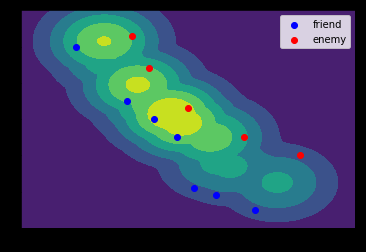
\includegraphics{state_no_battle_prob.png}
\caption{战役发生概率密度分布}
\label{fig:stateNoBattleProb}
\end{figure}


显然这个概率分布的形状并不是哪种已知解析形式,从而从它中采样变成了个难题。 
这里使用所谓格采样法解决这个问题,考虑到这个问题的维度并不高。本例中,首先限制
密度的非零区域只取在 $[-1,5] \times [0,6]$上。
然后等距取$100 \times 100$个点作为对应小区域之密度的近似,
然后转为一个此区域所具有的离散概率所对应的随机变量。
一个采样率更小粒度更大的示意图可见于图~\ref{fig:gridify}。


\begin{figure}[htb]
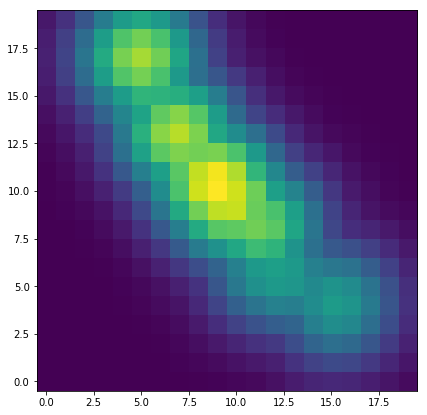
\includegraphics[width=0.6\linewidth]{gridify.png}
\caption{$25 \times 25$ 离散近似}
\label{fig:gridify}
\end{figure}


给出离散近似后,首先按离散概率从此二维网格中选一个格子,然后加上均匀分布噪声 
$dX \sim U(0,5-(-1)/100),dY \sim U(0,(6-0)/100)$ ,算出随机到的位置。

重复此过程10次,就可以从这个分布中采样到10个独立的样本,一个特定样本见图~\ref{fig:stateSampleBattle}。


\begin{figure}[htb]
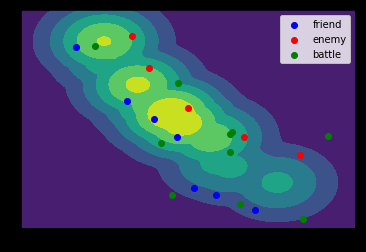
\includegraphics[width=0.6\linewidth]{state_sample_battle.png}
\caption{敌友军,战役概率与一个特定战役样本}
\label{fig:stateSampleBattle}
\end{figure}


这时如果把敌人的位置隐去,就可以得到实际推断中所用的数据,如图~\ref{fig:stateNoEnemy}。
类似频率主义稻草人式讨论,可以通过比较生成过程隐去的真实值与推断的值来判定推断的效能。

\begin{figure}[htb]
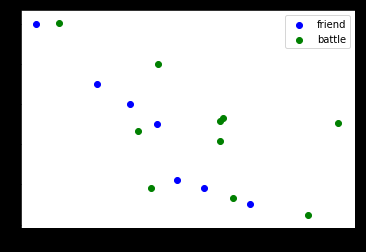
\includegraphics[width=0.6\linewidth]{state_no_enemy.png}
\caption{隐藏敌人后,实际推断时所能看到的信息}
\label{fig:stateNoEnemy}
\end{figure}

\subsection{另一种模型设定}


尽管这个分布看上去好像还不错,但是$\min$函数使得之后将介绍的三种基于梯度下降的方法无法发挥作用。
如考虑一个敌军备选点,如果并没有任何战役点的最近敌军点是它,则它并不能接收到任何梯度信息,
从而无法被优化。所以这里再建立另一种模型:

首先选择一个可微分分类器,它输入友军和敌军位置,
判别一个坐标点属于友军和敌军(注意友军和敌军也只有坐标信息)的概率。显然那些难以判别的点
可以被看做冲突可能最大的点,从而可以如此定义坐标$(x,y)$的冲突水平因子:

$$
P_{\text{conflict}}(x,y) = P_\text{ally}(x,y) P_\text{enemy}(x,y) = P_\text{ally}(x,y)(1-P_\text{ally}(x,y))
$$


这里$P_\text{ally}(x,y)$表示点$(x,y)$被分类器分类为友军的概率。

本文剩余内容使用朴素贝叶斯分配器作为分类器($x,y$坐标为独立的特征)。
它相对容易计算,其意义也易于解释。分类器分类概率被定义为:

$$
P_\text{ally}(x,y) = \frac{
N(x\mid \mu^A_X ,\sigma^A_X) N(y \mid \mu^A_Y, \sigma^A_Y)
}{
N(x \mid \mu^A_X , \sigma^A_X) N(y \mid \mu^A_Y , \sigma^A_Y) + 
N(x \mid \mu^E_X , \sigma^E_X) N(y \mid \mu^E_Y , \sigma^E_Y)
}
$$


这里$N(x \mid \mu,\sigma)$是正态分布概率密度分布函数:
$$
N(x \mid \mu,\sigma) = \frac{1}{\sqrt{2\pi \sigma^2}} \exp\left(\frac{(x-\mu)^2}{2\sigma^2}\right)
$$


分类器所用的参数$\mu,\sigma$以标准的矩估计法估计得到:

\begin{align*}
\mu_Z^S    &= 1/N^S \sum_{i=1}^N Z_i^S \\
\sigma_Z^S &= 1/N^S (Z_i^S - \mu_Z^S)^2
\end{align*}


这里 $Z \in \{ X,Y \}$ ,$S \in \{ A,E \}$。而 $N_S$为$S$方的单位数量。

图~\ref{fig:naivebayes} 可视化了各点的分类概率情况。

\begin{figure}[htb]
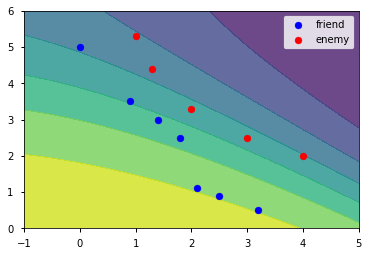
\includegraphics[width=0.6\linewidth]{naivebayes.png}
\caption{朴素贝叶斯分配器预测概率等高线图}
\label{fig:naivebayes}
\end{figure}


接下来,定义距离因子吸收回之前模型的距离信息。点与最近的单位的距离越小,则越有可能产生一场战斗,
定义为:

$$
P_{\text{distance}}(x,y) = \exp(-\alpha \min_{u} distance)
$$


这里$u$意为任意单位。$\min_u distance$所有单位所在点到点$(x,y)$之间的距离中最短者。

故而产生战斗概率为:

$$
P(x,y) = P_{\text{conflict}}(x,y) P_{\text{distance}}(x,y) = 
P_\text{ally}(x,y) P_\text{enemy}(x,y) \exp(-\alpha \min_{u} distance)
$$


设$\alpha=0.1$,这个二维函数值可见图~\ref{fig:combOne}:

\begin{figure}[htb]
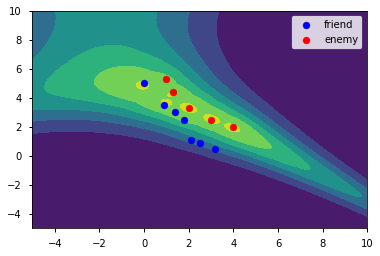
\includegraphics[width=0.6\linewidth]{comb1.png}
\caption{
组合朴素贝叶斯分类器与平滑的距离因子后的战斗发生概率}
\label{fig:combOne}
\end{figure}

光滑化概率虽然看起来不错,但是经过实验发现抽出来的样本有点过于分散了(见图~\ref{fig:combTwo})
而如果将考虑区域加大,则情况会变得更糟(见图~\ref{fig:combThree})。
虽然作者尝试调整参数设定,但没能达成两全其美。故而这个光滑设法只能又被放弃。
下面转而采用将冲突水平和距离直接与对应阈值比较,若没超过就直接设其概率为0的截断式设定。

\begin{figure}[htb]
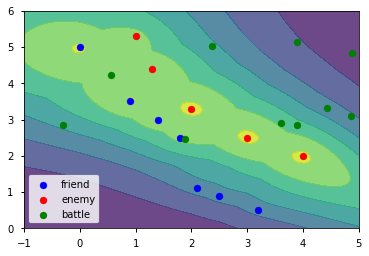
\includegraphics[width=0.6\linewidth]{comb2.png}
\caption{过于分散的样本}
\label{fig:combTwo}
\end{figure}

\begin{figure}[htb]
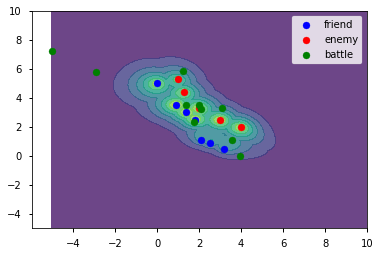
\includegraphics[width=0.6\linewidth]{comb4.png}
\caption{
当扩大讨论范围后,不合理的样本不可避免地出现}
\label{fig:combThree}
\end{figure}

\subsection{使用的基线模型}

$$
P(x,y) \propto
\begin{cases}
1 & P_\text{ally}(x,y) (1-P_\text{ally}(x,y)) > ct \quad \text{and} \quad \min_{u} distance < dt \\
0 & \text{otherwise}
\end{cases}
$$

这里$ct$是冲突水平阈值,而$dt$是距离阈值。后面取$ct=0.2,dt=1.0$。

图~\ref{fig:combFive}展示了样本点被强制落在阈值确定的区域内,解决了过于分散的困境。

\begin{figure}[htb]
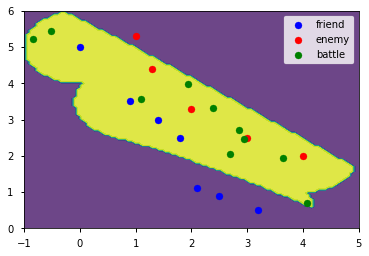
\includegraphics[width=0.6\linewidth]{comb5.png}
\caption{
强制0概率可以解决不合理点的麻烦}
\label{fig:combFive}
\end{figure}


不过这个设定同样有无法传递梯度信息问题,这里采用机器学习常用的“软化”方法(如机器学习把ReLu换成softplus)
来截断函数转为S型函数,这里采用sigmoid函数 $sigm(x) = \frac{1}{1+\exp(-x)}$:

$$
P(x,y) \propto sigm(t (P_\text{ally}(x,y) (1-P_\text{ally}(x,y)) - \theta_0)) sigm(t(-\min_{u} distance + \theta_1))
$$


这里 $t$ 是“紧绷度”参数,其控制了sigmoid函数的陡度, $\theta_0,\theta_1$是冲突程度和距离的阈值。
 设 $\theta_0=0.2,\theta_1=1.5,t = 10.0$,其效果可见图~\ref{fig:combSix}.


\begin{figure}[htb]
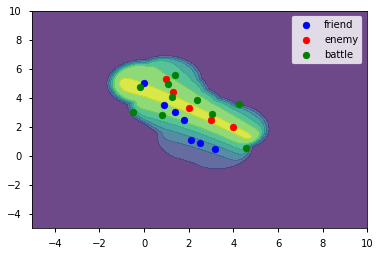
\includegraphics[width=0.6\linewidth]{comb6.png}
\caption{基线模型}
\label{fig:combSix}
\end{figure}


后文将使用这个模型和参数设定作为基线模型。

\clearpage
\section{推断的算法和框架}


\subsection{既有的推断框架}

贝叶斯推断框架是组织模型设定和推断方法的库或者领域特定语言。
现在已经很多流行的推断框架,如 Stan \cite{carpenter2017stan},
pymc\cite{patil2010pymc} , edward \cite{tran2016edward}. 
它们的核心是其所基于的自动求导库,这三个对别对应于 stan-math,theano,tensorflow。

其中Stan提供了一个新的DSL,但是编译太慢且难以调试,而且过于强调各个借口一致,其主推MCMC的历史
导致其变分推断的输出居然也是以样本表格格式输出的(为了与cmdStan一致),后来虽然以蹩脚的csv注释
方式给出了一些参数,但依然不能不利用hack获取协方差矩阵的信息。而pymc与edward都基于python,
但是为了强调灵活性大量不进行封装而直接调用theano和tensorflow的函数,这导致使用它们必须
了解这两个并不容易理解的库的背景知识(尤其是tensorflow),而光论灵活它的顶层API设计方式
又使它不那么灵活,这一点只要看看它的混合模型蹩脚的写法就可以认识到。

\subsection{推断方法和算法介绍}

这节将介绍三种后文反复使用的推断方法。本文为了回避上述框架的弱点,
并发挥推断的灵活(其实是为了自己实现算法加深理解,肯定不会继续用这个库)
自己开发了一个被称作bayes-torch的基于pytorch作为自动求导库的派生库,
\footnote{代码已托管在GitHub并发布在PyPi,
参见\url{https://github.com/yiyuezhuo/bayes-torch}, \url{https://pypi.org/project/bayes-torch/}},
实现了这三个方法。

\subsubsection{最大后验估计}


最大后验估计(MAP)找到使得似然函数和先验概率最大化的点作为估计值。由于梯度计算可以用pytorch自动完成,
这里只需调用SGD或者pytorch提供的其他面向神经网络的优化器(毕竟pytorch本身是用来实现动态神经网络的)
来进行标准的梯度下降(取 $loss = -likelihood \times prior$)过程。见算法~\ref{alg:sgd}。

\begin{algorithm}
\caption{随机梯度下降}
\begin{algorithmic}[1]
\Procedure{SGD}{$\theta,lr,step$} \Comment{$\theta$ 是初始值, $lr$ 更新速率,$step$ 是迭代步数}
    \For{i in 1:step}
        \State $\nabla \gets (\nabla_\theta \log(x,\theta)|_{\theta})$
        \State $\theta \gets \theta - lr \nabla -\theta$
    \EndFor
    \State \textbf{return} $\theta$
\EndProcedure
\end{algorithmic}
\label{alg:sgd}
\end{algorithm}

\subsubsection{变分推断}


变分推断使用简单的分布区近似复杂的精确后验分布。
它的优化目标是使得变分(近似)分布与原分布的Kullback-Leibler(KL)散度最小化
\cite{blei2017variational},KL散度定义为:

$$
KL(q||p) = E_q \left( \log \frac{q(\theta \mid \mu,\omega)}{p(\theta \mid x)} \right)
$$


这里$p(\theta \mid x)$是精确后验分布。$q(\theta)$(忽略优化参数$\mu,\omega$)是对应的近似精确分布的近似分布。
$q(\theta)$的分布族经常为了计算方便而选为正态分布,即$N(\mu,\mathbf{\Sigma})$形式。
如果协方差矩阵可以视作对角矩阵,即$\mathbf{\Sigma}=\mathrm{diag}(\exp(\mathbf{\omega}))$,
这就是所谓采用了平均场(meanfield)设定的变分推断(ADVI还有个满秩设定这里没有实现),
它在也许不合理的移去随机参数之间的关系的同时也极大减少了参数个数,加速了算法。

由于采用了近似分布而非精确后验分布作为权重计算期望(即计算$E_{q(\theta)}$而非$E_{p(\theta \mid x)}$),
解析上的计算难度下降了。不过$p(\theta \mid x)$显然还是没法算(本来就是近似目标)。
不过可以通过拿掉一个与目标无关常数因子绕过去,这个变化等价于最大化证据下界($\mathrm{ELBO}$)。
它的下界之名得自它是$\log p(x)$的下界:

\begin{align*}
\log p(x) &= \log \int_\theta p(x,\theta) = \log \int_\theta p(x,\theta) \frac{q(\theta)}{q(\theta)} = \log \left( E_q \frac{p(x,\theta)}{q(\theta)} \right)  \\
          &\ge E_q (\log p(x,\theta)) - E_q(\log q(\theta)) = \mathrm{ELBO}
\end{align*}


KL散度和ELBO的关系如下:

\begin{align*}
KL(q(\theta) || p(\theta \mid x)) &= E_q \log \frac{q(\theta)}{p(\theta \mid x)}  \\
                                  &= E_q \log q(\theta) - E_q \log p(\theta \mid x) \\
                                  &= E_q \log q(\theta) - E_q \log p(\theta,x) + E_q \log p(x) \\
                                  &= -(E_q \log p(\theta,x) -E_q \log q(\theta)) + \log p(x) \\
                                  &= -\mathrm{ELBO} + \log p(x)
\end{align*}


所以可以最大化ELBO来最小化KL散度。这个东西已经可以用类似上面的格点法近似计算,但维度一般太高无法处理。

而做这个优化的传统变分推断算法,类似EM算法的所谓的坐标提升变分推断(CAVI)算法
要求解析地计算条件期望$E_{-j}(\log p(\theta_j \mid \mathbf{\theta}_{-j},\mathbf{x}))$。
这并不是个如同自动求导一样容易自动解决的问题,这使得变分推断没有采样法这种某种意义上的黑箱方法一样流行。

为了回避解析计算,\cite{kucukelbir2017automatic}与\cite{kucukelbir2014fully}提出自动微分变分推断(ADVI)。
这个算法的核心是用蒙特卡洛法而非解析地计算期望$E_q(\cdot)$,如算法~\ref{alg:advi}所示。该算法是
\cite{kucukelbir2017automatic}的算法的简化版本,
简化掉的部分是原文讨论的针对更一般的非自由取值变量的变换的相应处理,由于本文不需要所以并没有被实现
(变换$\sigma=\exp(\omega)$除外,当然这个在原始算法里也没算作变换的一部分)。
另外就是本来算法有个类似动量优化算法的项,本文和bayes-torch简化成了固定步长梯度下降以便调试。

\begin{algorithm}
\caption{自动微分变分推断(平均场,不考虑变换)}
\begin{algorithmic}[1]
\Procedure{ADVI}{$\mathbf{\mu},\mathbf{\omega},lr,M,step$}  \Comment{$\mathbf{\mu},\mathbf{\omega}$ 是初始值,$M$是随机积分采样个数}
    \For{$s$ in $1:step$}
        \State $\hat{\nabla}_\mathbf{\mu} \gets \mathbf{0}$
        \State $\hat{\nabla}_\mathbf{\omega} \gets \mathbf{0}$
        \For{$i$ in $1:M$} 
            \State $\mathbf{\eta} \sim N(\mathbf{0},\mathbf{I}) $ \Comment{从多元标准正态分布中采样,下同}
            \State $\hat{\theta} \gets (\mathbf{\eta} * \exp(\mathbf{\omega})) + \mathbf{\mu}$ \Comment{$*$即按元素对应相乘}
            \State $\hat{\nabla}_\mathbf{\mu} \gets \hat{\nabla}_\mathbf{\mu} + (\nabla_\theta \log p(x,\theta)|_{\hat{\theta}})$
            \State $\hat{\nabla}_\mathbf{\omega} \gets \hat{\nabla}_\mathbf{\omega} + \hat{\nabla}_\mu * \mathbf{\eta}$
        \EndFor
        \State $\hat{\nabla}_{\mathbf{\mu}} \gets \hat{\nabla}_{\mathbf{\mu}} / M$
        \State $\hat{\nabla}_{\mathbf{\omega}} \gets (\hat{\nabla}_\mathbf{\omega} / M) * \exp(\mathbf{\omega}) + \mathbf{1}$
        \State $\mathbf{\mu} \gets \mathbf{\mu} + lr \hat{\nabla}_{\mathbf{\mu}}$
        \State $\mathbf{\omega} \gets \mathbf{\mu} + lr \hat{\nabla}_{\mathbf{\omega}}$
    \EndFor 
    \State \Return $\mathbf{\mu},\mathbf{\omega}$
\EndProcedure
\end{algorithmic}
\label{alg:advi}
\end{algorithm}


ADVI使用带噪声的梯度找到后验期望这一部分有点像降低效率版的MAP,不过这个噪声降低了期望的“估计效率”
的同时也提供了将(正态近似下的)方差参数连结进梯度的机会。

本文使用平均场设定后,后验概率看起来像:

$$
p(x^E_1,\dots,x^E_{N_E},y^E_1,\dots,y^E_{N_E} \mid D) \sim 
N((\mu_{X^E_1},\dots,\mu_{y^E_{N_E})^T},\mathrm{diag}(\sigma_{X^E_1},\dots,\sigma_{y^E_{N_E}}))
$$


条件独立性蕴含$p(x^E_i \mid D) \sim N(\mu_{x^E_i},\sigma_{x^E_i}^2)$,
其中$D$指模型中的已知数据,即给定的友方军队位置和战役位置。而诸如$\mu_{x^E_i},\sigma_{x^E_i}$
被称为变分(参数精确后验分布的近似分布的)参数。

\subsubsection{采样法}


变分推断只是近似方法,从后验分布中直接采样开销很大但是是精确方法(虽然它的保证收敛并没有看上那么有用)。
经典的Hasting-Metropolis法要使用手动指定的proposed分布,而且收敛效率不佳。哈密顿蒙特卡洛
(HMC,\cite{hoffman2014no},见算法~\ref{alg:hmc})效率更高,且不需要受手动指定proposed分布之苦,
符合各框架劝诱的黑箱统计风格。

\begin{algorithm}
\caption{哈密顿蒙特卡洛采样}
\begin{algorithmic}[1]
\Procedure{HMC}{$\theta_0,\epsilon,L,step$} \Comment{$L$ ,$\epsilon$ 是 leap-frog过程的参数}
    \For{$i$ in $1:step$}
        \State $r_0 \sim N(0,I)$
        \State $\theta_i \gets \tilde{\theta} \gets \theta_{i-1}$
        \State $\tilde{r} \gets r_0$
        \For{$l$ in $1:L$} \Comment{leap-frog过程}
            \State $\tilde{r} \gets \tilde{r} + (\epsilon/2) \nabla_\theta P(X,\theta)|_{\tilde{\theta}}$
            \State $\tilde{\theta} \gets \tilde{\theta} + \epsilon \tilde{r}$
            \State $\tilde{r} \gets \tilde{r} + (\epsilon/2) \nabla_\theta P(X,\theta)|_{\tilde{\theta}}$
        \EndFor
        \State $\alpha \gets \min \left\{ 1, \frac{\exp(P(x,\tilde{\theta})-\frac{1}{2}\tilde{r}\cdot\tilde{r})}{\exp(P(x,\theta_{i-1})-\frac{1}{2}r_0\cdot r_0)} \right\}$  \Comment{接受率,转移概率}
        \State $u \sim \mathrm{Uniform}(0,1)$
        \If{$u \le \alpha$}
            \State $\theta^i \gets \tilde{\theta}$
        \EndIf
    \EndFor
    \State \Return $\theta$
\EndProcedure
\end{algorithmic}
\label{alg:hmc}
\end{algorithm}


HMC使用与ADVI类似的利用梯度冲击和震荡收集方差信息。

HMC和其他采样法会返回随机游走轨道,这个轨道可以近似的看做精确后验分布的采样样本,所以可以用来计算
其他参数或者生成经验分布函数之类的。后文并不会利用采样法的精确特征,
基本只用上它的期望和方差,作类似于ADVI的解释。

\clearpage
\section{推断实验}

\subsection{敌军位置探测}


如图~\ref{fig:expState}所示的局势会被用在接下来的推断实验中。

\begin{figure}[htb]
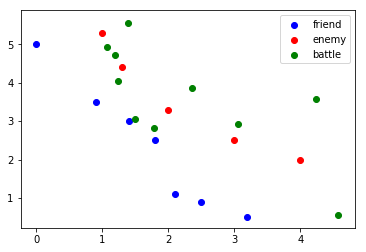
\includegraphics[width=0.6\linewidth]{exp_state.png}
\caption{Given situation}
\label{fig:expState}
\end{figure}


\subsubsection{MAP}


首先,如果使用均匀先验(等价于只有似然函数起作用),MAP的估计结果可见于图~\ref{fig:MAPone}。

\begin{figure}[htb]
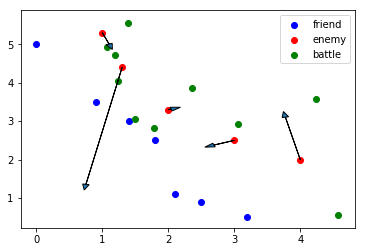
\includegraphics[width=0.6\linewidth]{MAP1.png}
\caption{均匀先验下的MAP}
\label{fig:MAPone}
\end{figure}


箭头尾指向对应敌军的“真实位置”(对推断来说不可见),箭头头指向MAP估计的敌军位置。正如所见,
有一个敌军单位的估计位置被拉到友军后方以最大化概率,这是很明显的过拟合的标志。
贝叶斯框架解决这种问题的标准方式就是引入先验
\footnote{或者叫机器学习的规范项之类的,但是看起来贝叶斯的概率解释更优雅一些。},如:

$$
P_{\text{enemy}}(x,y) = \exp(sigm(t((x+y) - \alpha)))
$$


这里$t$是敌军位置的紧绷度参数。$\alpha$是对应的阈值。这里设$t=5.0,\alpha=5.0$。

由于该先验给敌军单位落在对角线右上的区域以偏好,所以称作对角先验。加上对角先验后的联合概率函数看起来像:

\begin{align*}
\log p(\mathbf{x}^E,\mathbf{y}^E) &= \sum_{i=1}^{N_B} \log sigm(t (P_\text{ally}(x^B_i,y^B_i)(1-P_\text{ally}(x^B_i,y^B_i)) - \theta_0)) \\
                                  &+ \sum_{i=1}^{N_B} \log sigm(t(-\min_{u} distance(x^B_i,y^B_i) + \theta_1)) \\
                                  &+ \sum_{j=1}^{N_E} sigm(t((x^E_j+y^E_j) - \alpha))
\end{align*}


这里$N_B,N_E$是战役和敌人单位的个数。$x^B_i,y^B_i$是第$i$个战役的坐标。$x^E_j,y^E_j$是第$j$个敌人的坐标。

从图~\ref{fig:MAPtwo}中可以看出,加上对角先验后的MAP结果不再出现那种过拟合情况。

\begin{figure}[htb]
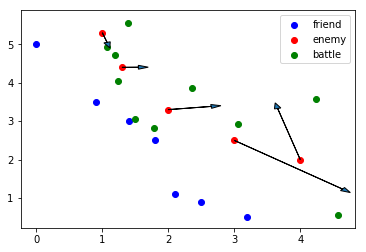
\includegraphics[width=0.6\linewidth]{MAP2.png}
\caption{对角先验下的MAP}
\label{fig:MAPtwo}
\end{figure}

\subsubsection{采样和变分推断}


点估计本身没有给出关于估计的不确定性信息。尽管精确后验分布的参数可以直接给出但是难以计算。
贝叶斯推断中两种解决方式就是采样和变分推断(VI)。前者产生一个与精确后验相关的随机游走轨迹,其可以看做
从后验中采样出来的,精确但是效率低下,而变分推断快得多但是理论上仅是近似。

分别采用均匀先验和对角先验两次变分推断拟合结果见图~\ref{fig:VI}。

分别采用均匀先验和对角先验两次采样结果见图~\ref{fig:samping}。

\begin{figure}[htb]
  \begin{subfigure}[b]{0.45\linewidth}
    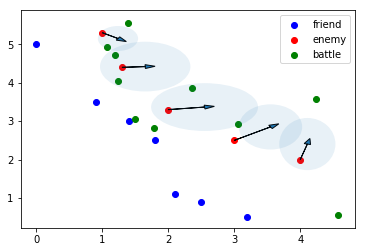
\includegraphics[width=\linewidth]{VI11.png}
    \caption{变分推断+均匀先验例一}
  \end{subfigure}
  \begin{subfigure}[b]{0.45\linewidth}
    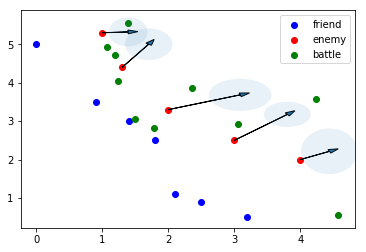
\includegraphics[width=\linewidth]{VI12.png}
    \caption{变分推断+对角先验例一}
  \end{subfigure}
  \begin{subfigure}[b]{0.45\linewidth}
    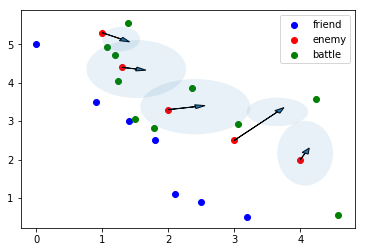
\includegraphics[width=\linewidth]{VI21.png}
    \caption{变分推断+均匀先验例二}
  \end{subfigure}
  \begin{subfigure}[b]{0.45\linewidth}
    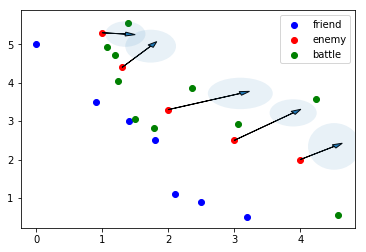
\includegraphics[width=\linewidth]{VI22.png}
    \caption{变分推断+对角先验例二}
  \end{subfigure}
  \caption{变分推断拟合结果}
  \label{fig:VI}
\end{figure}

\begin{figure}[htb]
  \begin{subfigure}[b]{0.45\linewidth}
    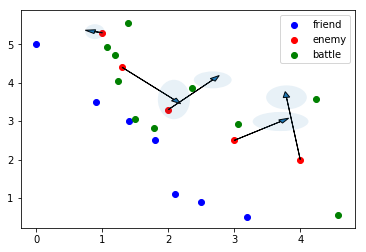
\includegraphics[width=\linewidth]{Sampling11.png}
    \caption{哈密顿蒙特卡洛+均匀先验例一}
  \end{subfigure}
  \begin{subfigure}[b]{0.45\linewidth}
    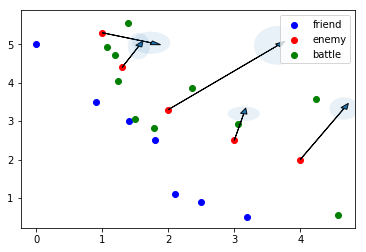
\includegraphics[width=\linewidth]{Sampling12.png}
    \caption{哈密顿蒙特卡洛+对角先验例一}
  \end{subfigure}
  \begin{subfigure}[b]{0.45\linewidth}
    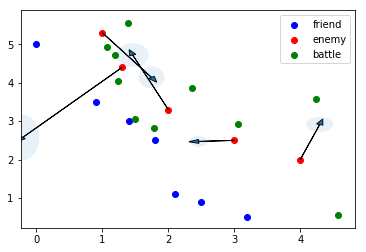
\includegraphics[width=\linewidth]{Sampling21.png}
    \caption{哈密顿蒙特卡洛+均匀先验例二}
  \end{subfigure}
  \begin{subfigure}[b]{0.45\linewidth}
    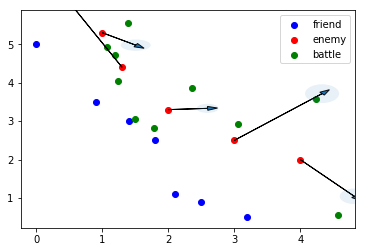
\includegraphics[width=\linewidth]{Sampling22.png}
    \caption{哈密顿蒙特卡洛+对角先验例二}
  \end{subfigure}
  \caption{采样法拟合结果(100次采样)}
  \label{fig:samping}
\end{figure}

图中的椭圆的中心表示拟合的后验分布(以参数化正态分布或轨迹的经验分布表示)$x,y$的期望,
椭圆的两轴长表示拟合的后验分布的$x,y$的标准差。故而这些椭圆可以看成对计算得近似后验分布的一个粗略表示,
之后将一直沿用这个表示方法。

图中可以看到哈密顿蒙特卡洛的拟合结果看起来不能保持一致,这意味着随机游走未充分收敛。
扩大样本量可以稍微解决这个问题(10倍样本结果见图~\ref{fig:SamplingTen})。但是即使是100个样本,
在作者的老爷机上都已经很慢了,所以后文使用的都是变分推断法,而不用采样法。

\begin{figure}[htb]
  \begin{subfigure}[b]{0.45\linewidth}
    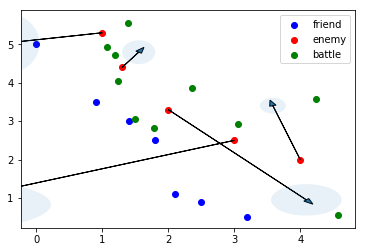
\includegraphics[width=\linewidth]{Sampling31.png}
    \caption{哈密顿蒙特卡洛+均匀先验例一}
  \end{subfigure}
  \begin{subfigure}[b]{0.45\linewidth}
    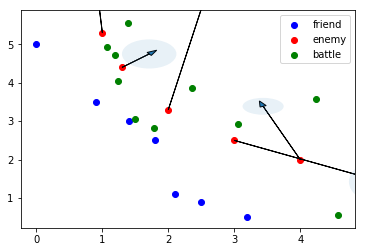
\includegraphics[width=\linewidth]{Sampling32.png}
    \caption{哈密顿蒙特卡洛+对角先验例一}
  \end{subfigure}
  \begin{subfigure}[b]{0.45\linewidth}
    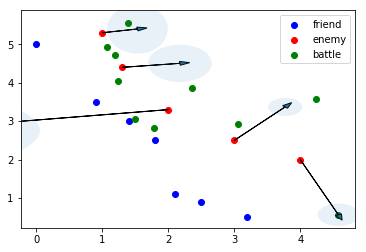
\includegraphics[width=\linewidth]{Sampling41.png}
    \caption{哈密顿蒙特卡洛+均匀先验例二}
  \end{subfigure}
  \begin{subfigure}[b]{0.45\linewidth}
    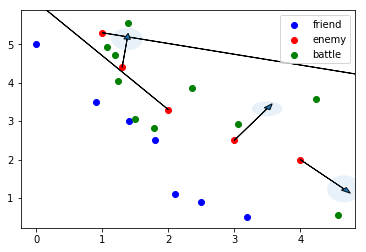
\includegraphics[width=\linewidth]{Sampling42.png}
    \caption{哈密顿蒙特卡洛+对角先验例二}
  \end{subfigure}
  \caption{采样拟合结果(1000次采样)}
  \label{fig:SamplingTen}
\end{figure}

\subsection{变化敌人数量设定}

上面的估计都基于已给定“真实”的敌人数量。为了讨论此算法的稳定性,特别是实际不知道敌人确切数量,
乃至给出的数量与实际数量偏差很大时,算法会给出什么结果?图~\ref{fig:bigVb}展示了不同数量设定下的
结果(初始值以真实值插值而来)。可见均匀先验的结果就看起来不错,而对角先验有点过于被先验支配了。
不过总的来说变化敌人数量反而可以证明本算法的有效性。

\begin{figure}[htb]
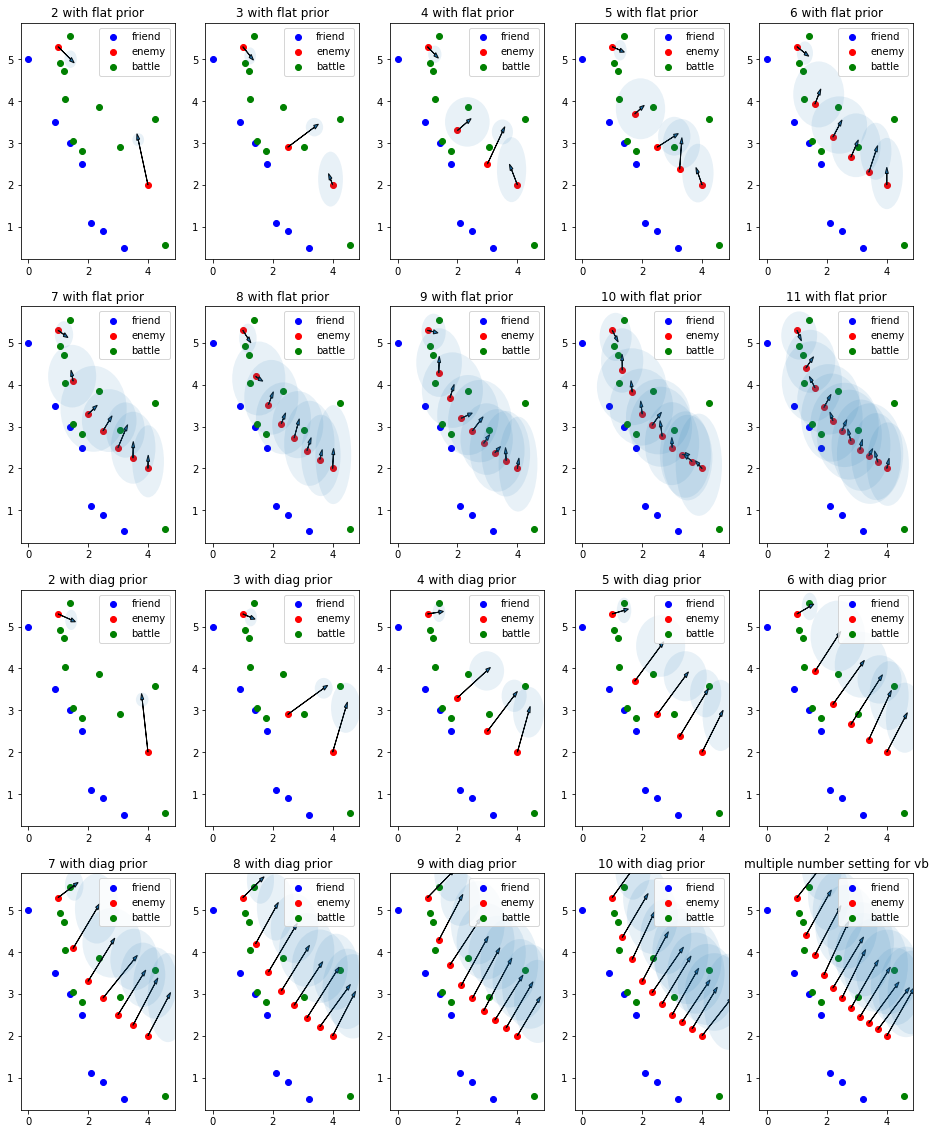
\includegraphics[width=0.99\linewidth]{big_vb.png}
\caption{变动数量时的近似结果}
\label{fig:bigVb}
\end{figure}

\subsubsection{敌人存在性概率密度估计}


这里采用正态分布族的变分推断的一大好处就是计算特定敌军单位在特定区域的后验概率十分方便。
从而可以直接计算出任意矩形区域$[x,x+dx]\times[y,y+dy]$中存在任意敌军单位的概率:

\begin{align*}
pe(x,y,dx,dy) = 1-
\prod_i^{N_E}
(1-
& ((\Phi((x + dx - \mu_{X^E_i})/\sigma_{X^E_i}) - \Phi((x - \mu_{X^E_i})/\sigma_{X^E_i})) \\
&  (\Phi((y + dy - \mu_{Y^E_i})/\sigma_{Y^E_i}) - \Phi((y - \mu_{Y^E_i})/\sigma_{Y^E_i})))
)
\end{align*}


这里$\Phi(x)$是标准正态分布累积分布函数:

$$
\Phi(x) = \int_{-\infty}^x \frac{1}{\sqrt{2\pi}} \exp\left(\frac{x^2}{2}\right)
$$


而$\mu_{X^E_i}$是第$i$个敌人的近似后验分布的正态期望参数,另外几个类似。

以此可以近似地计算定义出存在密度:

$$
pe(x,y) = pe(x-\epsilon,y-\epsilon,2\epsilon,2\epsilon)/(4 \epsilon^2)
$$


其中$\epsilon$是一个足够小的数,在这取$\epsilon=0.01$。两个数量设定的计算的结果
可见于等高线图~\ref{fig:existDensity}。类似上面比较各个数量的结果见图~\ref{fig:bigVbExist}。

\begin{figure}[htb]
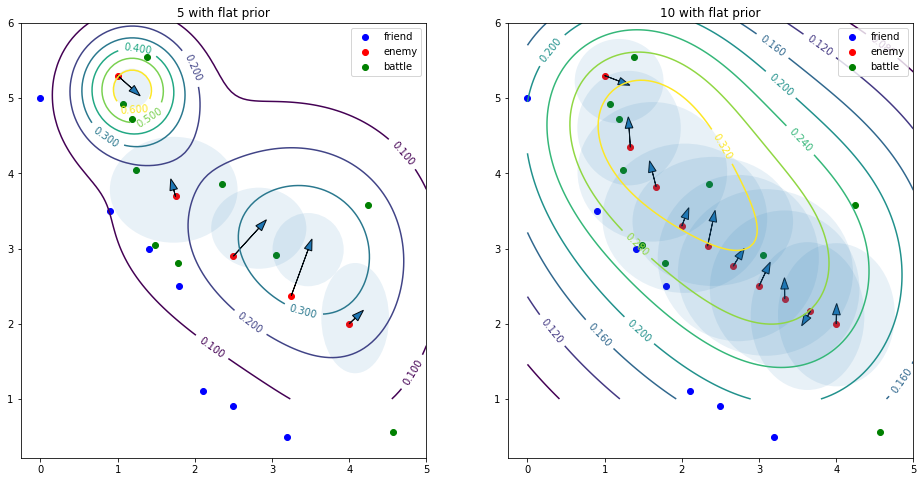
\includegraphics[width=0.99\linewidth]{exist_density.png}
\caption{两个数量设定下的存在概率密度估计}
\label{fig:existDensity}
\end{figure}


\begin{figure}[htb]
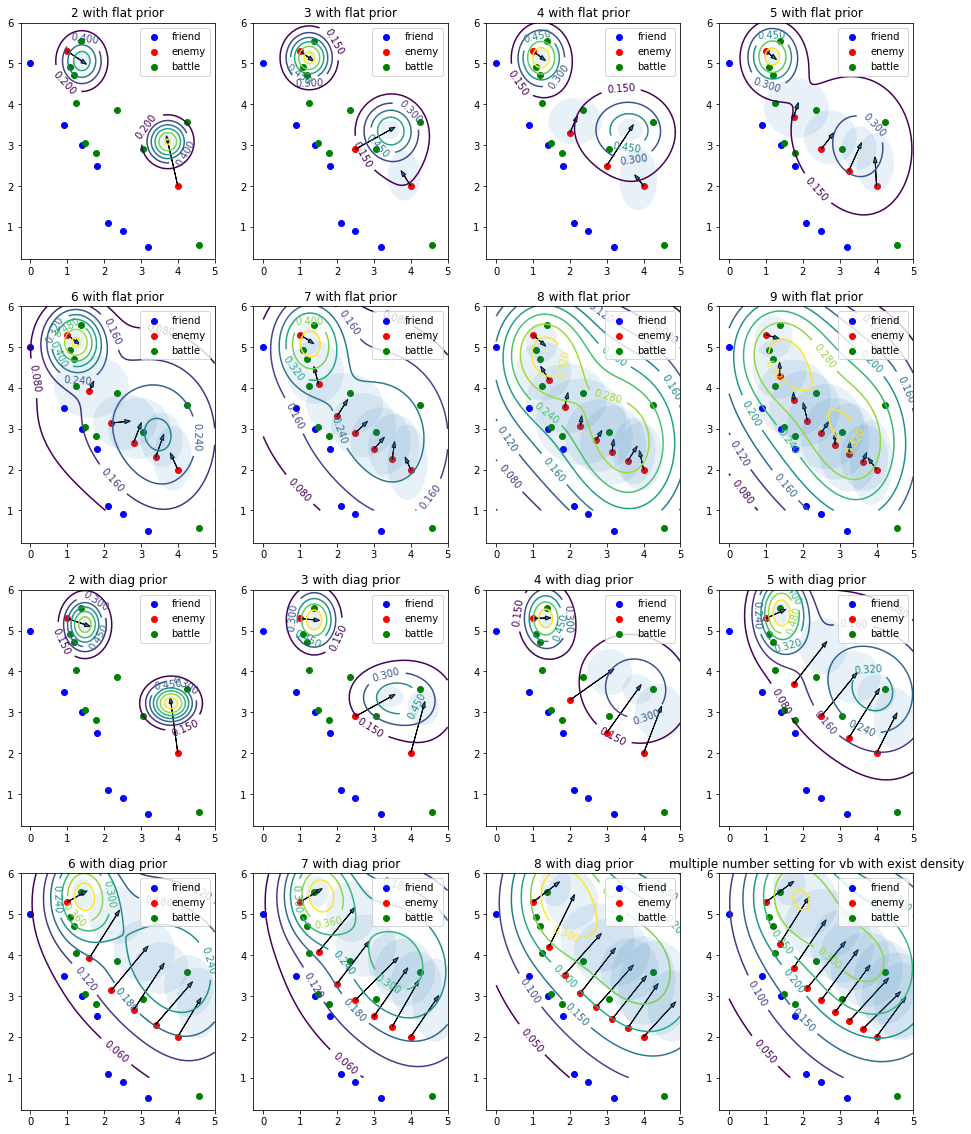
\includegraphics[width=0.99\linewidth]{big_vb_exist_prob.png}
\caption{多个数量设定下的存在概率估计}
\label{fig:bigVbExist}
\end{figure}


\clearpage
\section{扩展:敌方运动侦测}


考虑友军,敌军,战役不仅有位置信息,还有关于何时在何地的时间信息,即敌友军可以在一个时间段内运动
并在一些时间发生战斗\footnote{这里发生时间和次数的随机过程化似乎更有必要了,然而为了简化这里两个都是给定的}
,如何推断运动呢?得益于模型的设定方式,仅需一点点改造以上模型就可以继续使用。

假定时间开始于$0$并终结于$1$,而敌我双方均以固定的速度(每个单位可以不同)进行匀速运动。故而之前的
参数$x^E_i$可被重写为$x^E_i(t) = (1-t)x^E_i(0) + tx^E_i(1)$。这里$x^E_i(0),x^E_i(1)$是取代原先参数的两个
新参数,表示敌人单位在时间0,1时的位置。其他的几个随机参数或数据也类似如此改变(友军被钦定了额外的运动方式,
在本例中友军都在向“前”运动)。

首先,假定敌军期初位置$x^E_i(0),y^E_i(0)$已知而末期位置$x^E_i(1),y^E_i(1)$未知,
推断的结果可见图~\ref{fig:bkeu}(所有点颜色深浅表示对应的时间,浅为较早)。这里箭头尾表示已知的初始点,
有椭圆包着的那个箭头头坐标表示估计的结果(类似前面,坐标指期望,长短半径场指两轴上的标准差)。
另外一个箭头是“真实”期末点。

\begin{figure}[htb]
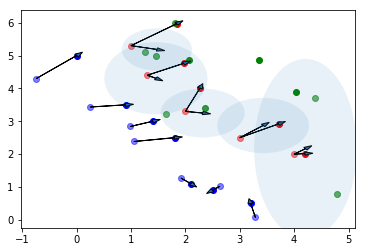
\includegraphics[width=0.4\linewidth]{bkeu.png}
\caption{运动推断:$t=0$已知而$t=1$未知}
\label{fig:bkeu}
\end{figure}


图~\ref{fig:bueu}显示了当$t=0,1$时敌人的位置都未知时的推断结果\footnote{注意它们没用同一个数据}。
连续的两个箭头的箭头尾出指向真实初始点,中点表示估计的期初点位置坐标的后验期望,
箭头头是估计的期末点位置坐标的后验期望。

\begin{figure}[htb]
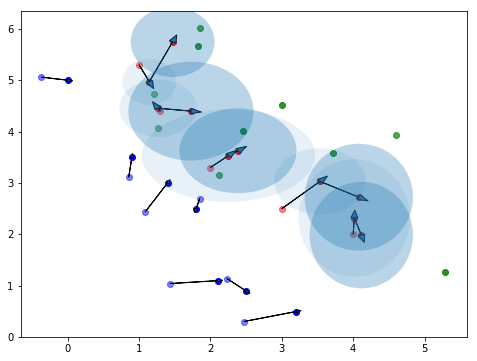
\includegraphics[width=0.6\linewidth]{bueu.png}
\caption{运动推断:$t=0$与$t=1$时敌人位置都未知}
\label{fig:bueu}
\end{figure}


注意这个模型对可能出现的超长运动没有进行先验的惩罚。由于算法在这个数据上效果还不错,
作者又没有很多空余时间,就没有专门构造个数据去验证这类先验设定的效果了。

\clearpage
\section{扩展:处理复杂的复杂的分布形状}


上面讨论的基本都基于那个很容易给出一条曲线将两组点分开的数据,
从而模型中插入的极其简化的朴素贝叶斯分类器都能充分发挥其效能。下面将测试一些其他的形状。

\subsection{圆形}


这里将友军位置设为圆形的,战役的位置设定成敌军将友军包围所可能产生的情况。由于敌军位置本身不给定,
从而迭代初始值不像之前那样设成真实值而设成随机值。如果这些点可以自动移动到外围的话,就可以看做验证了
算法的有效性。而迭代结果如图~\ref{fig:circleIteration}所示,仅仅需要均匀先验而不需要给定
敌军在外部的先验就可以收敛到比较恰当的位置上。

\begin{figure}[htb]
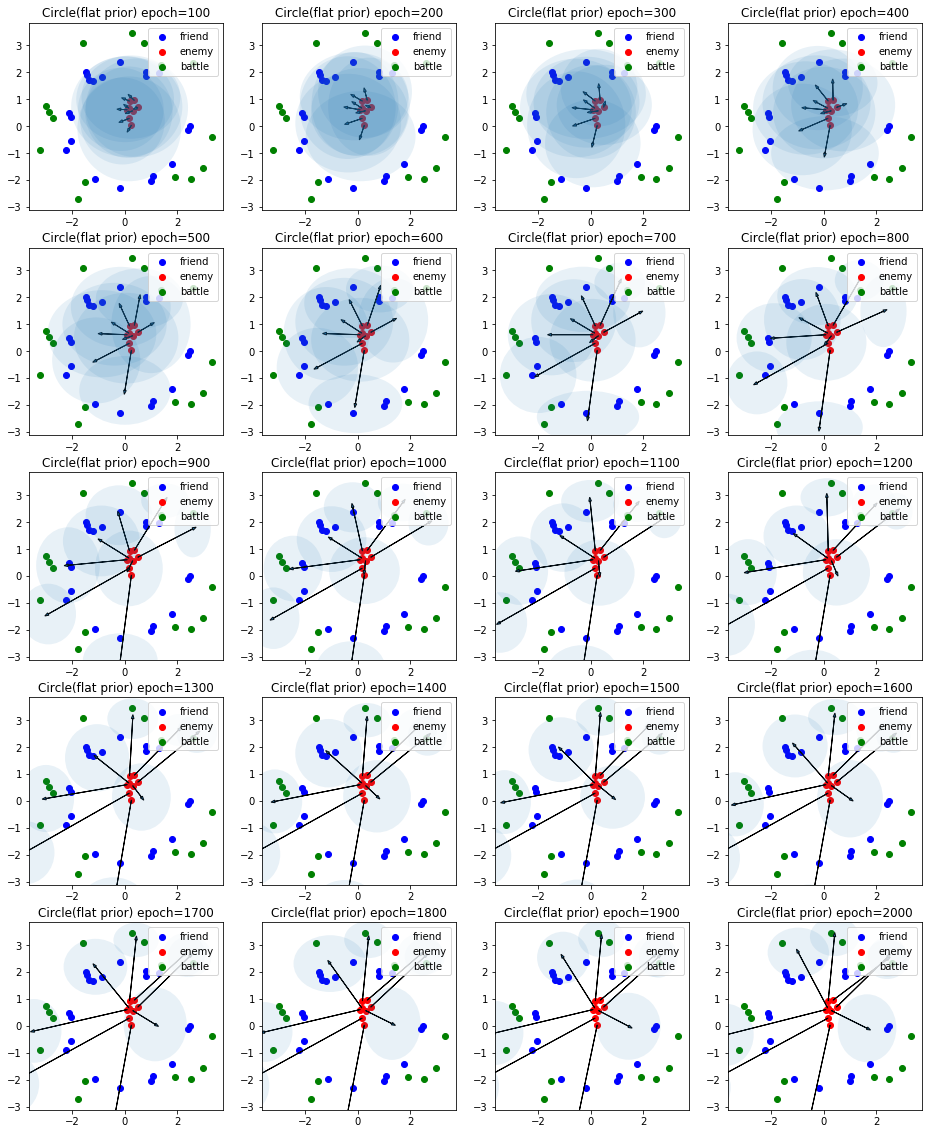
\includegraphics[width=0.99\linewidth]{circle_iteration.png}
\caption{
均匀先验+圆形设定+随机初始化下的迭代收敛过程}
\label{fig:circleIteration}
\end{figure}

\subsection{案例研究:葛底斯堡战役}


本节不再使用前面使用的真空中的球形鸡来验证模型,而直接使用真实战例的数据。图~\ref{fig:gettysburg}
展示了葛底斯堡战役第二天的战场示意图和单位相对位置数据
数据分别标出了旅级单位的分布和师级单位的分布\footnote{位置是其实HPS提供的剧本初始时旅长师长的位置,
显然HPS研究人员自己也不清楚这些人当时确切在哪,而只是根据他们的历史研究常识选择了他们认为的最恰当的点。
本文相当于借助了他们的常识},
下面的推断使用师级单位,放出旅级的图是因为看起来更连续一些\footnote{你可能会注意到两图在右上角并不完全一致,
这是因为战场示意图是战斗过程的图,而散点图则是机动到进攻阵地前的确切位置}。数据来自HPS兵棋
“内战系列:葛底斯堡”,此外还有一个人数表,见表~\ref{tab:Confederate}与表~\ref{tab:Union}。
人数将作为后面的将人数考虑进来的模型的权重。另外可从人数上看出联邦军的师规模比南方邦联军小,
所以对所有单位使用相同的参数可能并不十分恰当(在前面时可以假定各单位同质回避这个问题,
然而这里显然不同质)。这问题将在下一节解决。

\begin{figure}[htb]
  \begin{subfigure}[b]{0.49\linewidth}
    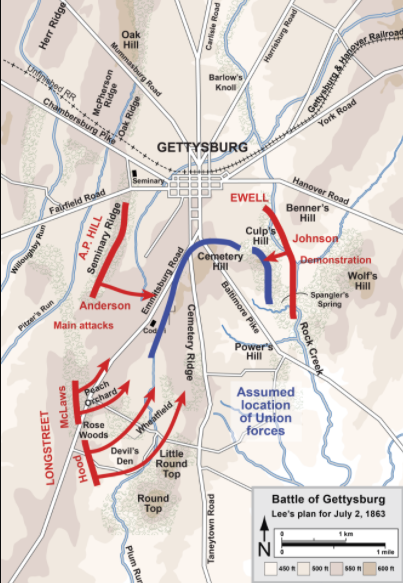
\includegraphics[width=\linewidth]{gettysburg-map.png}
    \caption{葛底斯堡战役第二天的战场示意图}
  \end{subfigure}
  \begin{subfigure}[b]{0.49\linewidth}
    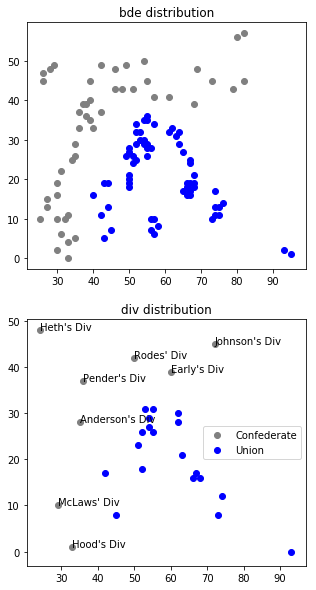
\includegraphics[width=\linewidth]{gettysburg-model.png}
    \caption{旅/师级单位位置坐标}
  \end{subfigure}
  \caption{真实情况和模型使用的数据的比较}
  \label{fig:gettysburg}
\end{figure}

\begin{table}[h]
\parbox{.45\linewidth}{
\caption{南方邦联军编制}
\begin{tabular}{lrrr}
\toprule
{} &  兵力 &    x &    y \\
\midrule
Heth's Div     &      4628 &  2.4 &  4.8 \\
McLaws' Div    &      6762 &  2.9 &  1.0 \\
Hood's Div     &      6957 &  3.3 &  0.1 \\
Anderson's Div &      6686 &  3.5 &  2.8 \\
Pender's Div   &      5080 &  3.6 &  3.7 \\
Rodes' Div     &      5202 &  5.0 &  4.2 \\
Early's Div    &      4572 &  6.0 &  3.9 \\
Johnson's Div  &      6012 &  7.2 &  4.5 \\
\bottomrule
\end{tabular}
\label{tab:Confederate}
}
\hfill
\parbox{.45\linewidth}{
\caption{联邦军编制}
\begin{tabular}{lrrr}
\toprule
{} &  兵力 &    x &    y \\
\midrule
2nd D (Humphreys)   &      4913 &  4.2 &  1.7 \\
1st Div (Birney)    &      5008 &  4.5 &  0.8 \\
2nd Div (Gibbon)    &      3558 &  5.1 &  2.3 \\
3rd Div (Hays)      &      3622 &  5.2 &  2.6 \\
1st Div (Caldwell)  &      3303 &  5.2 &  1.8 \\
3rd Div (Schurz)    &      1633 &  5.3 &  3.1 \\
2nd Div (Steinwehr) &      2264 &  5.4 &  2.9 \\
3rd Div (Doubleday) &      2922 &  5.4 &  2.7 \\
1st Div (Barlow)    &      1475 &  5.5 &  3.1 \\
2nd Div (Robinson)  &      1311 &  5.5 &  2.6 \\
1st Div (Wadsworth) &      1697 &  6.2 &  3.0 \\
2nd Div (Geary)     &      3851 &  6.2 &  2.8 \\
1st Div (Williams)  &      4698 &  6.3 &  2.1 \\
2nd Div (Ayres)     &      3990 &  6.6 &  1.6 \\
1st Div (Barnes)    &      3411 &  6.7 &  1.7 \\
3rd Div (Crawford)  &      2842 &  6.8 &  1.6 \\
3rd Div (Newton)    &      4729 &  7.3 &  0.8 \\
1st Div (Wright)    &      4181 &  7.4 &  1.2 \\
2nd Div (Howe)      &      3548 &  9.3 &  0.0 \\
\bottomrule
\end{tabular}
\label{tab:Union}
}
\end{table}


下面假定联邦军的位置已知而南方邦联军的位置位置(即南方邦联军等价于前面的敌军)。

图~\ref{fig:gettysburgTwo}展示了给定两军位置时正向生成模型给出的战役发生概率密度。

\begin{figure}[htb]
  \begin{subfigure}[b]{0.49\linewidth}
    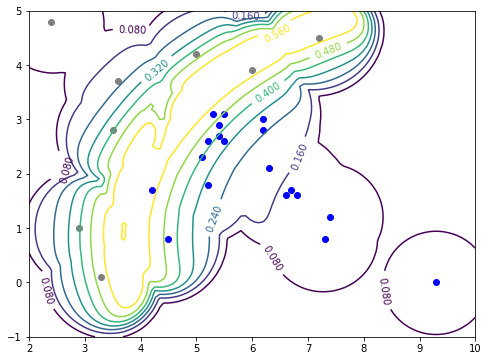
\includegraphics[width=\linewidth]{gettysburg-forward.png}
    \caption{未标准化的战役发生概率}
  \end{subfigure}
  \begin{subfigure}[b]{0.49\linewidth}
    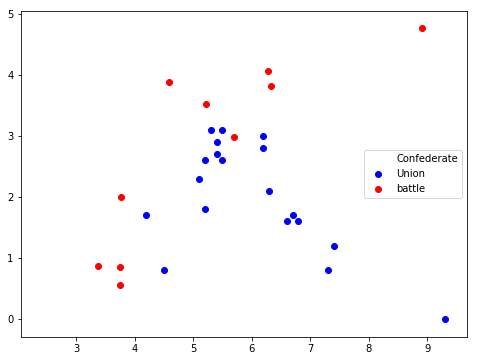
\includegraphics[width=\linewidth]{gettysburg-sample.png}
    \caption{一次采样结果+友军位置构成的模型所用数据}
  \end{subfigure}
  \caption{正向生成模型与一次采样结果}
  \label{fig:gettysburgTwo}
\end{figure}


这里仍采用随机初始化验证算法有效性,随机初始点设在左上角,若算法正常运行应该收敛到与真实点接近
的位置上。迭代过程和每个阶段的存在概率密度可见于图~\ref{fig:gettysburgInit}。

\begin{figure}[htb]
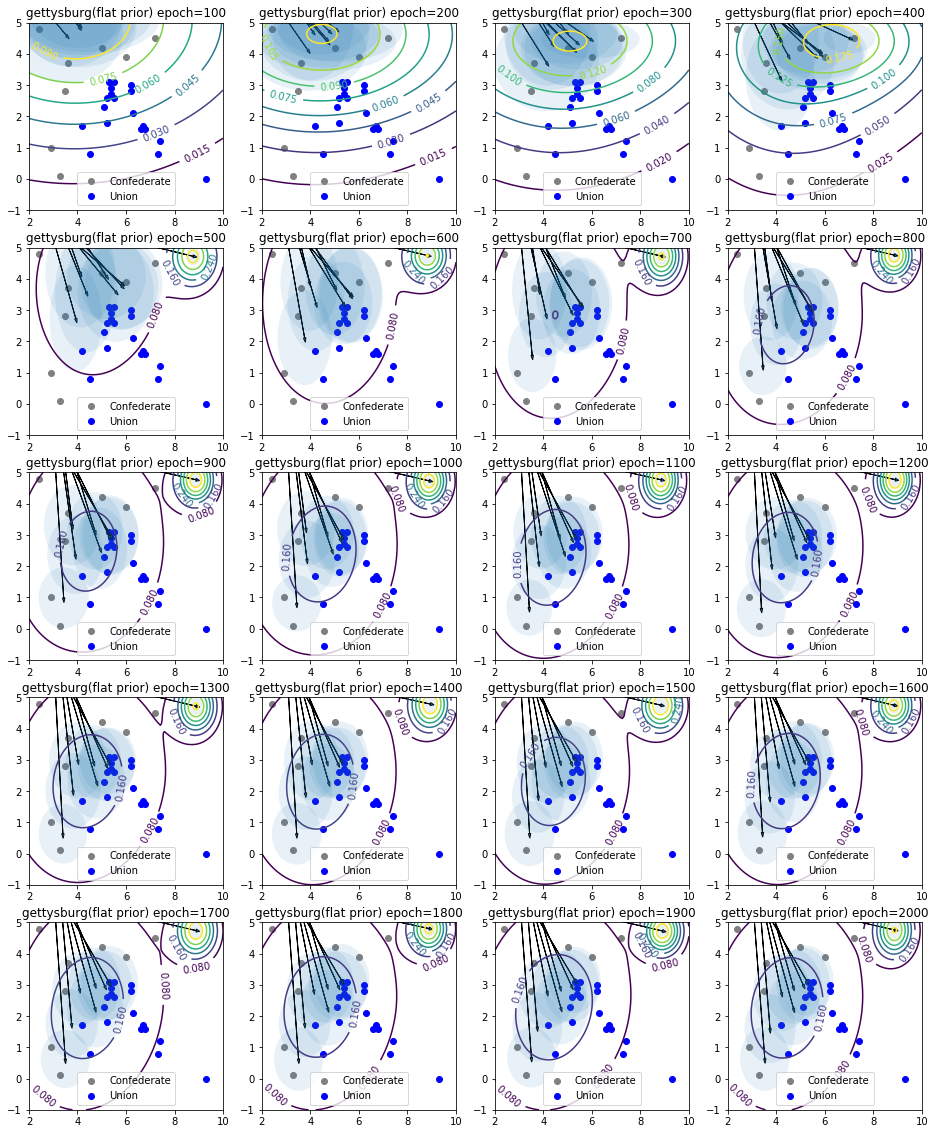
\includegraphics[width=0.99\linewidth]{gettysburg-init.png}
\caption{
均匀先验+随机初始化变分推断在葛底斯堡数据上的迭代过程}
\label{fig:gettysburgInit}
\end{figure}


拟合结果看上去还行,尽管敌军单位比起真实位置有点过于接近友方单位了,这个可以通过加先验惩罚解决。
不过比起在环上加环不如先把太阳当做中心。

\clearpage
\section{扩展:考虑规模效应模型}


前面的部分都假定战役和单位是同质的。但是上面的葛底斯堡战役例子明显违反了这个假设,
若能整合单位的规模(战斗力,影响辐射范围)信息进入模型,拟合结果应该会更好。

假定单位拥有越高的权重,则它的等效距离更短,同时在中心估计中的权重更大。

权重就使用表~\ref{tab:Confederate}与表~\ref{tab:Union}中的人数作为权重。贝叶斯分类器所用的
$\mu,\sigma$转而以加权方式计算。而距离则计算调整过的等效距离替代之前的距离,设:
$dist_{ij} = dist_{ij} \frac{\beta}{stre_i}$,其中参数$\beta$在此设为$6000$。这意味着所有的
联邦单位在距离影响上被惩罚了而一部分南方邦联单位在等效距离上得到了加成。

图~\ref{fig:gettysburgInitTwo}显示了拟合结果。它很类似于没有考虑规模效应的模型的拟合结果。
这可能是因为本例中各单位规模差距并没有大到产生显著影响的程度。另外这个设定本身也有一致性问题,
考虑几个处在同一格的单位似乎应该与一个有人数为它们之和的单位落在那的效果一致,但本模型设定下
只有在中心估计上一致,等效距离上却是不一致的,这个问题在联邦军左上角师级单位密集布防的区域
显得很明显。

\begin{figure}[htb]
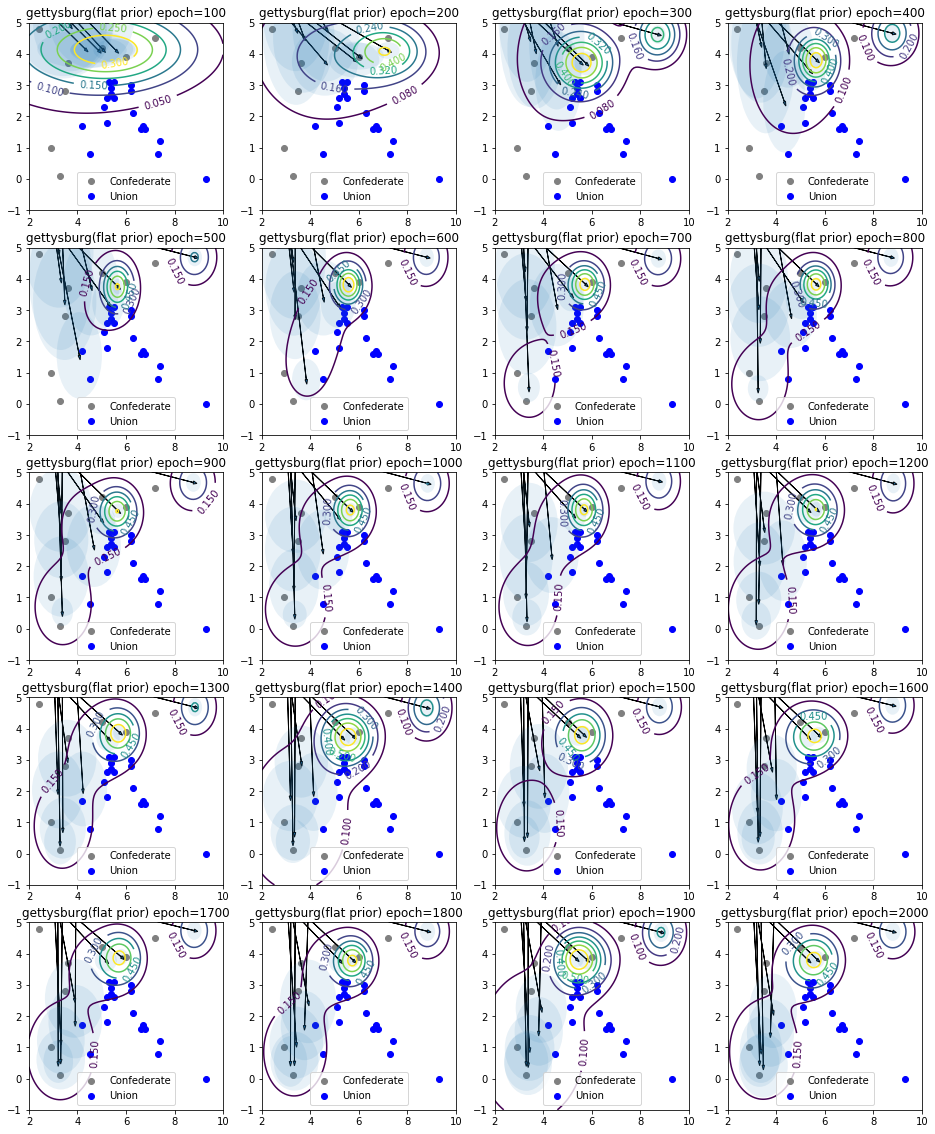
\includegraphics[width=0.99\linewidth]{gettysburg-init2.png}
\caption{
规模效应+随机初始化+均匀先验的迭代过程}
\label{fig:gettysburgInitTwo}
\end{figure}

\clearpage
\section{结论}

本文作者基于pytorch实现了一个贝叶斯推断框架bayes-torch并用它进行了相关实验推断。
推断主要包括敌人位置,运动轨迹,存在密度的推断,分别在均匀先验和问题特定先验,真实位置初始化,
多值插值初始化,多值随机初始化的情况下验证了算法的效果。并可以运用到相关侦测问题上。

写作本文的本来目的就是为作者准备设计的一个信息屏蔽为特点的游戏做准备,不过从实际效果来看
迭代速度过慢,老要钦定参数和分类器不能自适应(Edward的贝叶斯化神经网络看上去效果不错,
不过怎么看都只会更慢而且难以解释,本文没有使用它)都是一个问题。

这几天edward概率推断那里又搞了个大新闻,pytorch的分布的原生支持还是那么烂,
看起来是时候弃坑回到edward了(作者在2017年统计建模的论文\cite{touhou}里用过edward,并“荣获”成功参与奖。)
不过作者多少从手动实现这里获取了点对原理的认识。或者写LaTeX模板的知识?。。

%\begin{comment}

%\bibliography{paper} 
%\bibliographystyle{ieeetr}
%\makebibliography{paper}
%由于要求作者年份式引用,为了用plainnat这个包由与学校的脑子例子兼容只能重新实现这个功能了

\clearpage

\addcontentsline{toc}{section}{参考文献}
\bibliography{paper} 
\bibliographystyle{apalike}



%\appendix

\clearpage

\addcontentsline{toc}{section}{附录}

{\bf 附录一}

\section*{实现模型的主要代码}

这里列举的代码仅包括最重要的那些,样板代码和琐碎的绘图与工作函数可见于
\footnote{\url{https://github.com/yiyuezhuo/Undergraduate-thesis/tree/master/notebook}}。



基线模型的最顶层定义代码(底层就是那些pytorch代码,忽略)

\begin{python}

# model
friend = Data(friend_point)
battle = Data(battle_point)
enemy = Parameter(enemy_point) # set real value as init value, though maybe a randomed init is more proper

logPC = Data(_logPC)

conflict_threshold = 0.2
distance_threshold = 1.0
tense = 10.0
alpha = 5.0
prior_threshold = 5.0
prior_tense = 5.0

def target():
    friend_enemy = torch.cat((friend, enemy),0)
    distance = cdist(battle, friend_enemy).min(dim=1)[0]
    

    mu = Variable(torch.zeros(2,2)) 
    sd = Variable(torch.zeros(2,2))
    
    mu[0,:] = friend.mean(dim=0)
    mu[1,:] = enemy.mean(dim=0)
    sd[0,:] = friend.std(dim=0)
    sd[1,:] = enemy.std(dim=0)
    
    conflict = torch.exp(norm_naive_bayes_predict(battle, mu, sd, logPC)).prod(dim=1)
    p = soft_cut_ge(conflict,conflict_threshold, tense = tense) * soft_cut_le(distance, distance_threshold, tense = tense)
    
    target= torch.sum(torch.log(p))
    return target

def target2():
    target1 = target()
    # location prior
    target2 = target1 + torch.sum(enemy.sum(dim=1))
    return target2

\end{python}


运动侦测模型变体:

\begin{python}
def target():
    target = Variable(torch.zeros(1))
    for i in range(battle_point.shape[0]):
        t = timestamp[i]
        friend = friend0*(1-t) + friend1*t
        enemy = enemy0*(1-t) + enemy1*t
        single_battle = torch.unsqueeze(battle[i],0) 
        
        friend_enemy = torch.cat((friend, enemy), 0)
        distance = cdist(single_battle, friend_enemy).min(dim=1)[0]
        
        mu = Variable(torch.zeros(2,2)) 
        sd = Variable(torch.zeros(2,2))

        mu[0,:] = friend.mean(dim=0)
        mu[1,:] = enemy.mean(dim=0)
        sd[0,:] = friend.std(dim=0)
        sd[1,:] = enemy.std(dim=0)

        conflict = torch.exp(norm_naive_bayes_predict(single_battle, mu, sd, logPC)).prod(dim=1)
        p = soft_cut_ge(conflict,conflict_threshold, tense = tense) * soft_cut_le(distance, distance_threshold, tense = tense)

        target+= torch.sum(torch.log(p))
    return target

\end{python}


规模加权模型变体:

\begin{python}
# model for forward
reset()

friend = Data(friend_point)
battle = Data(xy)
enemy = Parameter(enemy_point) # set real value as init value, though maybe a randomed init is more proper

enemy_weight = Data(Confederate_weight)
friend_weight = Data(Union_weight)
enemy_dist_factor = Data(Confederate_dist_factor)
friend_dist_factor = Data(Union_dist_factor)


logPC = Data(_logPC)

conflict_threshold = 0.2
distance_threshold = 1.0
tense = 10.0
alpha = 5.0
prior_threshold = 5.0
prior_tense = 5.0

def target_p():
    friend_enemy = torch.cat((friend, enemy),0)
    friend_enemy_dist_factor = torch.cat((friend_dist_factor,enemy_dist_factor),0)
    
    distance = (cdist(battle, friend_enemy)*friend_enemy_dist_factor).min(dim=1)[0]
    #distance = distance * friend_enemy_dist_factor

    mu = Variable(torch.zeros(2,2)) 
    sd = Variable(torch.zeros(2,2))
    '''
    mu[0,:] = friend.mean(dim=0)
    mu[1,:] = enemy.mean(dim=0)
    sd[0,:] = friend.std(dim=0)
    sd[1,:] = enemy.std(dim=0)
    '''
    _friend_weight = torch.unsqueeze(friend_weight,1)
    _enemy_weight  = torch.unsqueeze(enemy_weight, 1)
    
    mu[0,:] = torch.sum(friend * _friend_weight,dim=0)
    mu[1,:] = torch.sum(enemy  * _enemy_weight, dim=0)
    sd[0,:] = torch.sqrt(torch.sum((friend - mu[0,:])**2 * _friend_weight, dim=0))
    sd[1,:] = torch.sqrt(torch.sum((enemy  - mu[1,:])**2 * _enemy_weight, dim=0))
    
    conflict = torch.exp(norm_naive_bayes_predict(battle, mu, sd, logPC)).prod(dim=1)
    p = soft_cut_ge(conflict,conflict_threshold, tense = tense) * soft_cut_le(distance, distance_threshold, tense = tense)
    return p

def target():
    p = target_p()
    
    target= torch.sum(torch.log(p))
    return target
    
# model for backward
reset()

friend = Data(friend_point)
battle = Data(battle_point)
enemy = Parameter(enemy_point) # set real value as init value, though maybe a randomed init is more proper

logPC = Data(_logPC)

conflict_threshold = 0.2
distance_threshold = 1.0
tense = 10.0
alpha = 5.0
prior_threshold = 5.0
prior_tense = 5.0


\end{python}


这里列举bayes-torch代码,Model类中包含本文中使用的三种推断算法的实现

\begin{python}

class Model:
    def __init__(self):
        self.parameters = []
        self.n_parameters = 0
        self.size_parameters = []
    def reset(self):
        self.parameters = []
        self.n_parameters = 0
        self.size_parameters = []
    def add_parameter(self, variable):
        self.parameters.append(variable)
        self.n_parameters += np.prod(variable.size())
        self.size_parameters.append(variable.size())
    def set_parameter_meanfield(self, mu, omega):
        n_parameters = self.n_parameters
        param_samples_eta = np.random.normal(size=n_parameters)
        param_samples = param_samples_eta*np.exp(omega) + mu
        self.set_parameter(param_samples)
        return param_samples_eta
    def set_parameter(self, values, is_float = True):
        # values is a flatten numpy array
        start = 0
        for param in self.parameters:
            param_size = np.prod(param.size())
            section = values[start:start+param_size].reshape(param.size())
            tensor = torch.from_numpy(section)
            if is_float:
                tensor = tensor.float()
            param.data = tensor
            start += param_size
    def collect_parameter_grad(self):
        grad = np.empty(self.n_parameters)
        start = 0
        for param in self.parameters:
            param_size = np.prod(param.size())
            grad[start:start+param_size] = param.grad.data.numpy().copy().ravel()
            start += param_size
        return grad
    def collect_parameter(self):
        res = np.empty(self.n_parameters)
        start = 0
        for param in self.parameters:
            param_size = np.prod(param.size())
            res[start:start+param_size] = param.data.numpy().copy().ravel()
            start += param_size
        return res
    def grad_q_meanfield(self, target_f, mu, omega, q_size=10, lr = 0.01):
        n_parameters = self.n_parameters
        
        mu_grad = np.zeros(n_parameters)
        omega_grad = np.zeros(n_parameters)
        
        optimizer = torch.optim.SGD(self.parameters, lr=lr)
        # optimizer only serve to zero_grad.
        
        for i in range(q_size):
            
            param_samples_eta = self.set_parameter_meanfield(mu, omega)
            
            optimizer.zero_grad()
            target = target_f()
            target.backward()
            
            param_grad = self.collect_parameter_grad()
            mu_grad += param_grad
            omega_grad += param_grad * param_samples_eta
        
        mu_grad /= q_size
        omega_grad /= q_size
        omega_grad *= np.exp(omega)
        omega_grad += 1.0
        
        return mu_grad,omega_grad
            
    def vb_meanfield(self, target_f, mu=None,omega=None, zero_init=False, 
                     n_epoch = 100, lr=0.01, q_size = 10):
        n_parameters = self.n_parameters
        
        if mu is None:
            if zero_init:
                mu = np.zeros(n_parameters)
            else:
                mu = np.array(self.collect_parameter())
        if omega is None:
            omega = np.zeros(n_parameters) # sigma=exp(omega) = 1
        
        #optimizer = torch.optim.SGD(self.parameters, lr=lr)
        
        for i in range(n_epoch):
            mu_grad,omega_grad = self.grad_q_meanfield(target_f, mu, omega, q_size = q_size)
            mu += lr * mu_grad
            omega += lr * omega_grad
        
        return mu,omega
        
        
    def vb_fullrank(self, target_f):
        raise NotImplementedError
    def vb_meanfield_format(self, res):
        # res = (mu, omega) -> {Parameter1: {'mu': mu1, 'sigma': exp(omega1)}...}
        mu, omega = res
        
        return_dict = {}
        start = 0
        for param in self.parameters:
            param_size = np.prod(param.size())
            _mu = mu[start:start+param_size].reshape(param.size())
            _omega = omega[start:start+param_size].reshape(param.size())
            return_dict[param] = {'mu':_mu,'omega':_omega}
            start += param_size
        return return_dict

    def vb(self, target_f, method = 'meanfield', format=False, 
                 reload=False, **kwargs):
        if method == 'meanfield':
            res = self.vb_meanfield(target_f, **kwargs)
            if not format:
                return res
            self.set_parameter(res[0])
            grad = self.grad(target_f) 
            grad_size = np.sum(grad**2)
            converge = grad_size < 0.01
            report = dict( method = 'meanfiled', 
                           est = self.vb_meanfield_format(res),
                           grad = grad,
                           grad_size = grad_size,
                           converge = converge)
            if reload:
                self.set_parameter(res[0])
            return report
        if method == 'fullrank':
            return self.vb_fullrank(target_f, **kwargs)
        raise NotImplementedError
    def sampling_hmc(self, target_f, epsilon=0.01, L=20, M=100):
        
        def grad(theta):
            self.set_parameter(theta)
            return self.grad(target_f)
        def likelihood(theta):
            self.set_parameter(theta)
            return target_f().data.numpy()
        
        sample =[]
        sample.append(self.collect_parameter())
        accept_list = []
        
        for m in range(M):
            r0 = np.random.normal(size=self.n_parameters)
            r = r0
            theta0 = sample[-1]
            theta = theta0.copy()
            
            for i in range(L):
                r = r + 0.5 * epsilon * grad(theta)
                theta = theta + epsilon * r
                self.set_parameter(theta)
                r = r + 0.5 * epsilon * grad(theta)
            odd_up = np.exp(likelihood(theta)-0.5*np.dot(r,r))
            odd_bottom = np.exp(likelihood(theta0)-0.5*np.dot(r0,r0))
            alpha = min(1,odd_up/odd_bottom)
            accept_list.append(alpha)
            
            if np.random.random() < alpha:
                sample.append(theta)
            else:
                sample.append(theta0)
        return sample
        

    def sampling(self, target_f, method= 'hmc', **kwargs):
        #trace = []
        #raise NotImplementedError
        if method == 'hmc':
            return self.sampling_hmc(target_f, **kwargs)
        if method == 'nuts':
            return self.sampling_nuts(target_f, **kwargs)
        raise NotImplementedError
    def optimizing(self, target_f, lr=0.01, n_epoch = 1000):
        '''
        After optimizing run, the result is stored in original torch variable.
        target_f don't have any parameter, since the class serve to delete the trouble
        '''
        optimizer = torch.optim.SGD(self.parameters, lr=lr)
        
        for epoch in range(n_epoch):
            optimizer.zero_grad()
            target = target_f()
            loss = -target
            loss.backward()
            optimizer.step()
    def grad(self, target_f):
        fake_lr = 1.0
        optimizer = torch.optim.SGD(self.parameters, lr=fake_lr)
        optimizer.zero_grad()
        target = target_f()
        target.backward()
        return self.collect_parameter_grad()

\end{python}


最相关的bayes-torch其他函数:

\begin{python}
def torch_norm_log_prob(X,mu,sd):    
    temp = -(X - mu)**2/(2*sd) 
    temp = temp - 0.5 * torch.log(2.0 * np.pi * sd)
    return temp

def torch_norm_naive_bayes_predict(X,mu,sd,logPC):
    # X: sample_size * features
    # mu: class_size * features
    # sd: class_size * featrues
    # log_PC class_size
    n_class = logPC.size()[0]
    n_feature = X.size()[1]
    n_sample = X.size()[0]
    _X = torch_tile(X,[1,n_class]).resize(n_sample,n_class,n_feature)
    cp = torch_norm_log_prob(_X, mu, sd).sum(dim=2) + logPC  
    log_predict_prob = torch_transpose((torch_transpose(cp) - torch_logsumexp(cp,dim=1)))
    return log_predict_prob
    
def torch_logsumexp(X,dim=0):
    # numpy have this function
    return torch.log(torch.exp(X).sum(dim=dim))

def torch_tile(X,repeats):
    # torch.repeat ~ numpy.tile
    return X.repeat(*repeats)


def torch_soft_cut_ge(x,threshold,tense=1.0):
    return torch.sigmoid(tense*(x-threshold))

def torch_soft_cut_le(x,threshold,tense=1.0):
    return torch.sigmoid(tense*(-x+threshold))


\end{python}

Notebook specific code, the density estimation:

Jupyter notebook实验中主要绘图和密度估计代码:

\begin{python}

def prob_point(x,y,dx,dy,_mu,_omega):
    mu = _mu.reshape(enemy_point.shape)
    sigma = np.exp(_omega.reshape(enemy_point.shape))
    x = np.reshape(x,(-1,1))
    y = np.reshape(y,(-1,1))
    px  = stats.norm.cdf((x-mu[:,0])/sigma[:,0])
    pdx = stats.norm.cdf((x+dx-mu[:,0])/sigma[:,0])
    py  = stats.norm.cdf((y-mu[:,1])/sigma[:,1])
    pdy = stats.norm.cdf((y+dy-mu[:,1])/sigma[:,1])
    return (pdx - px) * (pdy - py)

def prob_exist(x,y,dx,dy,_mu,_omega):
    ememy_prob = prob_point(x,y,dx,dy,_mu,_omega)
    return 1-np.prod((1 - ememy_prob).T,axis=0) 

def prob_exist_limit(x,y,_mu,_omega,step=0.1):
    p = prob_exist(x-step,y-step,2*step,2*step,_mu,_omega)
    return p/(4*step*step)

def show_change(show=False):
    display_data()
    for i in range(enemy_point.shape[0]):
        #s = 0.1
        plt.arrow(enemy_point[i][0], enemy_point[i][1], enemy.data[i][0] - enemy_point[i][0], enemy.data[i][1] - enemy_point[i][1],head_width=0.1)
    plt.legend()
    if show:
        plt.show()


def show_ellipse(mu,sd):
    from matplotlib.patches import Ellipse
    
    #ax = plt.subplot(111)
    ax = plt.gca() # get current axe, the lame method to support command style
    show_change(show=False)
    #res_reshaped = [r.reshape(enemy_point.shape) for r in res]
    for i in range(enemy_point.shape[0]):
        mu_x,mu_y = mu[i]
        sd_x,sd_y = sd[i]
        e=Ellipse((mu_x,mu_y), sd_x, sd_y, 0)
        e.set_clip_box(ax.bbox)
        e.set_alpha(0.1)
        ax.add_artist(e)
        
    #plt.show()
    
    
def show_vb(vb_res):
    res = vb_res
    model.set_parameter(res[0])
    res_reshaped = [r.reshape(enemy_point.shape) for r in res]
    mu = res_reshaped[0]
    sd = np.exp(res_reshaped[1])
    show_ellipse(mu,sd)
    
def multi_enemy_setting_show_exist_density(_enemy_point, target, title_string):
    reset_enemy(_enemy_point)
    res = vb(target)
    show_vb(res)
    p_exist = prob_exist_limit(xy[:,0],xy[:,1],res[0],res[1],step=0.001).reshape(xx.shape)
    CS = plt.contour(xx,yy,p_exist)
    #plt.contour(xx, yy, p_exist)
    plt.clabel(CS)
    #plt.title(title_string.format(i))
    plt.gca().set_title(title_string.format(i))
    plt.legend()

    
    
plt.figure(figsize=(16,20)) #(x,y)
for i in range(2, 10):
    interp_x = np.linspace(_enemy_point[:,0].min(),_enemy_point[:,0].max(),i)
    interp_y = np.interp(interp_x, _enemy_point[:,0], _enemy_point[:,1])
    interp_xy = np.c_[interp_x,interp_y]
    plt.subplot(4, 4, i-1)
    multi_enemy_setting_show_exist_density(interp_xy, target , '{} with flat prior')

for i in range(2, 10):
    interp_x = np.linspace(_enemy_point[:,0].min(),_enemy_point[:,0].max(),i)
    interp_y = np.interp(interp_x, _enemy_point[:,0], _enemy_point[:,1])
    interp_xy = np.c_[interp_x,interp_y]
    plt.subplot(4, 4, 8+i-1)
    multi_enemy_setting_show_exist_density(interp_xy, target2 , '{} with diag prior')

    #multi_enemy_setting_show(interp_xy, target2, '{} with diag prior')
plt.title('multiple number setting for vb with exist density')
plt.show()


\end{python}



\end{document}